\documentclass[12pt,]{article}
\usepackage[left=1in,top=1in,right=1in,bottom=1in]{geometry}
\newcommand*{\authorfont}{\fontfamily{phv}\selectfont}
\usepackage[]{mathpazo}


  \usepackage[T1]{fontenc}
  \usepackage[utf8]{inputenc}




\usepackage{abstract}
\renewcommand{\abstractname}{}    % clear the title
\renewcommand{\absnamepos}{empty} % originally center

\renewenvironment{abstract}
 {{%
    \setlength{\leftmargin}{0mm}
    \setlength{\rightmargin}{\leftmargin}%
  }%
  \relax}
 {\endlist}

\makeatletter
\def\@maketitle{%
  \newpage
%  \null
%  \vskip 2em%
%  \begin{center}%
  \let \footnote \thanks
    {\fontsize{18}{20}\selectfont\raggedright  \setlength{\parindent}{0pt} \@title \par}%
}
%\fi
\makeatother




\setcounter{secnumdepth}{0}


\usepackage{graphicx,grffile}
\makeatletter
\def\maxwidth{\ifdim\Gin@nat@width>\linewidth\linewidth\else\Gin@nat@width\fi}
\def\maxheight{\ifdim\Gin@nat@height>\textheight\textheight\else\Gin@nat@height\fi}
\makeatother
% Scale images if necessary, so that they will not overflow the page
% margins by default, and it is still possible to overwrite the defaults
% using explicit options in \includegraphics[width, height, ...]{}
\setkeys{Gin}{width=\maxwidth,height=\maxheight,keepaspectratio}


 



\author{}


\date{}

\usepackage{titlesec}

\titleformat*{\section}{\normalsize\bfseries}
\titleformat*{\subsection}{\normalsize\itshape}
\titleformat*{\subsubsection}{\normalsize\itshape}
\titleformat*{\paragraph}{\normalsize\itshape}
\titleformat*{\subparagraph}{\normalsize\itshape}





\newtheorem{hypothesis}{Hypothesis}
\usepackage{setspace}


% set default figure placement to htbp
\makeatletter
\def\fps@figure{htbp}
\makeatother

\usepackage{hyperref}
\setlength\parindent{24pt}
\usepackage{multirow}
\usepackage{helvet}
\usepackage{setspace}
\renewcommand\familydefault{\sfdefault}
\usepackage{fullpage}
\usepackage{pdflscape}
\usepackage{booktabs}
\usepackage{longtable}
\usepackage{array}
\usepackage{multirow}
\usepackage{wrapfig}
\usepackage{float}
\usepackage{colortbl}
\usepackage{pdflscape}
\usepackage{tabu}
\usepackage{threeparttable}
\usepackage{threeparttablex}
\usepackage[normalem]{ulem}
\usepackage{makecell}
\usepackage{xcolor}

% move the hyperref stuff down here, after header-includes, to allow for - \usepackage{hyperref}

\makeatletter
\@ifpackageloaded{hyperref}{}{%
\ifxetex
  \PassOptionsToPackage{hyphens}{url}\usepackage[setpagesize=false, % page size defined by xetex
              unicode=false, % unicode breaks when used with xetex
              xetex]{hyperref}
\else
  \PassOptionsToPackage{hyphens}{url}\usepackage[draft,unicode=true]{hyperref}
\fi
}

\@ifpackageloaded{color}{
    \PassOptionsToPackage{usenames,dvipsnames}{color}
}{%
    \usepackage[usenames,dvipsnames]{color}
}
\makeatother
\hypersetup{breaklinks=true,
            bookmarks=true,
            pdfauthor={},
             pdfkeywords = {},  
            pdftitle={},
            colorlinks=true,
            citecolor=blue,
            urlcolor=blue,
            linkcolor=magenta,
            pdfborder={0 0 0}}
\urlstyle{same}  % don't use monospace font for urls

% Add an option for endnotes. -----


% add tightlist ----------
\providecommand{\tightlist}{%
\setlength{\itemsep}{0pt}\setlength{\parskip}{0pt}}

% add some other packages ----------

% \usepackage{multicol}
% This should regulate where figures float
% See: https://tex.stackexchange.com/questions/2275/keeping-tables-figures-close-to-where-they-are-mentioned
\usepackage[section]{placeins}


\begin{document}
	
% \pagenumbering{arabic}% resets `page` counter to 1 
%    





\vskip -8.5pt


 % removetitleabstract

\noindent \doublespacing 

\pagebreak

\setlength{\parindent}{0in}
\setlength{\leftskip}{0in}
\setlength{\parskip}{8pt}
\vspace*{-0.2in}

\noindent

\textbf{Testing MaxEnt model performance in a novel geographic region
using an intentionally introduced insect}

Sutton, G. F.\textsuperscript{1}\(\dag\); Martin,
G.D.\textsuperscript{1,2}

\hfill\break

\begingroup
\fontsize{10}{12}\selectfont

\textsuperscript{1} Center for Biological Control, Department of Zoology
and Entomology, Rhodes University, Makhanda, 6140, South Africa

\textsuperscript{2} Afromontane Research Unit and Department Zoology and
Entomology, University of the Free State, Phuthaditjhaba, 9866, South
Africa \endgroup

\hfill\break

\textbf{Corresponding author} \(\dag\)
\href{mailto:g.sutton@ru.ac.za}{\nolinkurl{g.sutton@ru.ac.za}}

\pagebreak

\setlength\parindent{24pt}

\hypertarget{abstract}{%
\section{Abstract}\label{abstract}}

Ecological models are important tools to support and guide the
development and implementation of environmental policies and management
programs. Species distributions models (SDM's), such as the popular
MaxEnt software, are frequently used to guide conservation programmes,
predict the potential distribution of invasive species, forecast the
impacts of climate change and develop applied ecological research
(e.g.~biological control). Many applications of these models require
that SDM's are transferred in either space and/or time. However, few
studies to date have tested the transferability, and thus usefulness, of
MaxEnt models using fully independent data. Moreover, numerous authors
have raised concerns over how model complexity (controlled primarily by
feature class and regularisation multiplier settings) may affect MaxEnt
model transferability. In this paper, we evaluated the usefulness of
MaxEnt models transferred in space using a native Australian insect,
\emph{Dasineura rubiformis} Kolesik (Diptera: Cecidomyiidae) that has
been intentionally introduced as a biological control agent of the
invasive plant, \emph{Acacia mearnsii} De Wild (Fabaceae) in South
Africa. MaxEnt models were developed using native-range records only
(Australia) and projected over South Africa to identify the potential
climatic suitability for the insect, using a range of model settings
configurations. Model transferability was assessed using independent
post-release data from South Africa. Our results demonstrated that
MaxEnt scores were positively correlated with increased establishment
rates for \emph{D. rubiformis} in South Africa. MaxEnt model outputs and
projections were relatively consistent, irrespective of the settings
used. Despite MaxEnt having to extrapolate over much of South Africa,
MaxEnt performance was higher than modelling climatic suitability as a
function of whether models were in extrapolation or interpolation. Our
study demonstrates that MaxEnt models can prove useful when transferred
in space, however, users need to be aware of the effect of different
model settings configurations and model extrapolation can have on model
transferability and usefulness in applied ecological settings. We
demonstrate how validating the \emph{D. rubiformis} MaxEnt models can be
used to guide the biological control of \emph{A. mearnsii} using
\emph{D. rubiformis}.

~

\setlength{\parindent}{0in}
\setlength{\leftskip}{0in}
\setlength{\parskip}{8pt}
\vspace*{-0.2in}

\noindent

\textbf{Keywords}: Species distribution model, biological control,
\emph{Acacia}, \emph{Dasineura rubiformis}, model complexity, model
transferability

\setlength\parindent{24pt}

\hypertarget{introduction}{%
\section{1. Introduction}\label{introduction}}

Ecological models are important tools to support and guide the
development and implementation of environmental policies and management
programs (Addison et al., 2013; Schuwirth et al., 2019). For example,
ecological models can be used for planning conservation programs (Guisan
et al., 2013), predicting the establishment of invasive species (Martin
et al., 2020), implementing biological control programmes (Mukherjee et
al., 2021), or forecasting species responses to environmental change
(Bocedi et al., 2014). Species distribution models (SDM's) are an
example of ecological models that have become increasingly popular in
recent years (Elith and Leathwick, 2009). SDM's typically take the form
of correlative or mechanistic models that relate species
presence/absences to environmental covariates to map habitats that may
be suitable for a taxon (Elith et al., 2011). The Maximum Entropy
Species Distribution Model (hereafter `MaxEnt') (Phillips et al., 2017)
is among the most popular methods for species distribution modeling and
has been shown to perform well compared to alternative modeling
algorithms (Elith et al., 2006). It uses maximum entropy to distinguish
between environmental conditions where the focal taxon is present from
environmental conditions at background locations where the taxons'
presence is absent (or assumed absent) (Elith et al., 2011).

Despite its popularity, the usefulness of MaxEnt has been questioned
when used to generate predictions for novel geographic regions
(transferred in space) or time periods (transferred in time) from those
for which the data used to build the model were collected (Blasi et al.,
2021; Yates et al., 2018). To date, studies assessing transferability
have produced contrasting results (Bahn and McGill, 2013; Capinha et
al., 2018; Randin et al., 2006). Model transferability has typically
been assessed by cross validation, whereby a fraction of the data is
withheld to calibrate the model (i.e.~training data) and the remaining
data is retained to validate the model (i.e.~the testing data) (Wenger
and Olden, 2012). However, cross validation may not provide an estimate
of model transferability as a selected test sample may not provide an
unbiased estimate of the full data set, and therefore may not reflect
the heterogeneity that may exist in the underlying data in space or time
(see Wenger and Olden, 2012). Ideally, a direct test of model
transferability should use an independent dataset of species
presence/absences and environmental covariates (Fielding and Bell, 1997;
West et al., 2016). Unfortunately, very few studies, to date, have
tested model transferability using independent datasets (e.g. Costa et
al., 2010; Rebelo and Jones, 2010), which may have limited our
understanding of how useful SDM's can be when transferred in space or
time. Issues with model transferability may lead to misleading
conclusions, which may hinder scientists abilities to address important
ecological questions (e.g.~where could an invasive species establish?,
where should a conservation priority be translocated?) (Merow et al.,
2013).

Model complexity can affect uncertainty of model transferability in
space and time (Warren et al., 2014). Model complexity may be affected
by numerous parameters, notably the feature classes and regularisation
(beta) multiplier settings used to specify the MaxEnt model (Elith et
al., 2011; Merow et al., 2013). MaxEnt allows users to specify
combinations of different feature classes that modify the shape and
complexity of species-environment functions. Moreover, MaxEnt uses a
regularisation multiplier (a form of L\textsubscript{1}-regularisation)
to balance model complexity with the model fit, penalising unnecessarily
complex models (Merow et al., 2013). The default MaxEnt settings use all
feature classes in model fitting except `threshold' features (depending
on sample size of training data) and a regularisation multiplier of 1
(Phillips et al., 2017). Several recent studies have highlighted the
importance of species-specific tuning of feature classes and
regularisation multipliers for optimising model complexity
(Radosavljevic and Anderson, 2014; Shcheglovitova and Anderson, 2013),
with default settings often producing models that are overly complex,
and thus, may perform poorly when transferred (Elith et al., 2011; Merow
et al., 2013). Despite the potential implications, surprisingly few
studies use user-defined feature class and regularisation settings (e.g.
Sutton, 2019), and as such, little is known about how model settings
configurations may influence model transferability (Low et al., 2021;
Moreno-Amat et al., 2015).

In this study, we performed a retrospective assessment of the
transferability of SDM's built using MaxEnt (Phillips et al., 2017).
Here, we modelled the potential climatic suitability of an insect that
is native to Australia, and that has been introduced into South Africa
as a biological control agent. The insect, \emph{Dasineura rubiformis}
Kolesik (Diptera: Cecidomyiidae) was introduced into South Africa from
Australia in 2001, and found to be established in 2006, to curb the
spread of the invasive Australian \emph{Acacia mearnsii} De Wild (Impson
et al., 2013). Extensive field surveys have been performed in Australia
(characterizing the native distribution of \emph{D. rubiformis}) (Adair,
2004) and long-term post-release monitoring has been performed in South
Africa to measure establishment rates of the insect, following
experimental releases of the insect (Impson et al., 2021). As such, the
availability of independent testing data from a separate continent to
the data used to generate the models makes this an ideal study system
for assessing the transferability of SDM's.

We built MaxEnt models for \emph{D. rubiformis} using distribution
records from its native distribution (Australia), and projected the
resulting MaxEnt suitability rasters over South Africa. MaxEnt scores
range from 0 to 100, whereby 0 represents regions predicted to be highly
unsuitable and 100 indicating highly suitable regions. To test model
transferability, we fit the MaxEnt scores as a covariate in a logistic
regression model to determine whether MaxEnt scores were statistically
relevant predictors of insect establishment rates in South Africa (with
these data being entirely independent of the data used to build the
MaxEnt models). A strong, positive correlation between MaxEnt scores and
insect establishment rates would provide support that the SDM's were
useful when transferred in space (from Australia to South Africa).
Moreover, we tested whether model complexity and parameter tuning could
improve the accuracy and transferability of MaxEnt by comparing the
predictive power of MaxEnt models calibrated with default settings and
an array of optimised settings configurations.

\hypertarget{methods-and-materials}{%
\section{2. Methods and Materials}\label{methods-and-materials}}

\hypertarget{species-occurences-records}{%
\subsection{2.1. Species occurences
records}\label{species-occurences-records}}

A total of 103 native-range records for \emph{D. rubiformis} were
obtained from Adair (2004). A total of 452 invaded-range records to
evaluate model transferability were taken from Impson, Kleinjan and
Hoffmann (unpublished). Distribution maps for \emph{D. rubiformis} for
both native and invaded range are provided in Fig. 1.

Spatial autocorrelation is an important factor that may affect model
outputs. Filtering of species occurrence data may limit the inherent
biases in the data and improve model quality (Veloz, 2009). To avoid
pseudo-replication, only one occurrence record per 2.5 minute grid cell
was used for model calibration. Species occurrence datasets were thinned
using the \texttt{spThin} package (Aiello-Lammens et al., 2015), and
spatial autocorrelation analyses were performed using the
\texttt{ecospat} package (Di Cola et al., 2017).

\hypertarget{environmental-predictors}{%
\subsection{2.2. Environmental
predictors}\label{environmental-predictors}}

Climate data were obtained by downloading the standard set of 19
bioclimatic variables from the WorldClim ver. 1.4 database (Hijmans et
al., 2005)\\
(data available at: www.worldclim.org/download.html). This dataset is
representative of annual and seasonal means and variation of temperature
and precipitation metrics averaged over the 1950--2000 time period
(current climate) at a 5 arc minute resolution.

To reduce multicollinearity between environmental predictors and thereby
decrease the risk of calibrating overfit models, Pearson's correlation
coefficients were computed for all pairs of predictors, whereby
predictors which were highly correlated (\textbar{}\emph{r}\textbar{}
\textgreater{} 0.85) were excluded from the final predictor set (Capinha
and Anastácio, 2011). The reduced set of environmental predictors
consisted of seven climatic variables, including: bio1 -- annual mean
temperature, bio2 -- mean diurnal temperature range (mean of monthly
{[}max temp -- min temp{]}, bio3 -- isothermality, bio9 -- mean
temperature of the driest quarter, bio12 -- mean annual precipitation,
bio14 -- precipitation of the driest month and bio16 -- precipitation of
the wettest quarter (see Hijmans et al. (2005) for further details).

\hypertarget{model-calibration}{%
\subsection{2.3. Model calibration}\label{model-calibration}}

Maxent was implemented in the \texttt{dismo} package in \texttt{R}
(Hijmans et al., 2017). MaxEnt was selected as it consistently
outperforms other modelling algorithms (Wisz et al., 2008). Given that
MaxEnt is a presence-only modelling algorithm, model calibration
requires a user-defined geographic background to sample the climate of
representative grid cells where the focal species is absent
(i.e.~background points). Background definition can have a significant
effect on model output (VanDerWal et al., 2009). The background should
ideally represent the geographic areas available to the focal species,
omitting areas where species absence is due to historical factors,
dispersal constraints and/or biotic interactions (Sanín and Anderson,
2018). Following Webber et al. (2011), we defined the model background
using the Koppen-Geiger climate classification (Available at:
\url{http://koeppen-geiger.vu-wien.ac.at}). Only Koppen-Geiger climate
zones that contained at least one native-range occurrence record for
\emph{D. rubiformis} were used as the background area from which
pseudo-absences were drawn for model calibration. Koppen-Geiger climate
zones were intersected using the \texttt{extract} function from the
\texttt{R} package \texttt{raster} (Hijmans et al., 2017).

\hypertarget{optimal-model-settings}{%
\subsection{2.4. Optimal model settings}\label{optimal-model-settings}}

Model performance and optimal settings configurations were assessed
using multiple metrics that reflected aspects of model (1)
discriminatory ability (AUC\textsubscript{test}), (2) overfitting
(AUC\textsubscript{diff}), (3) omission rates (OR\textsubscript{10}),
and (4) overall parsimony (AICc) (Low et al., 2021).

\begin{enumerate}
\def\labelenumi{(\arabic{enumi})}
\item
  AUC\textsubscript{test} assesses the models ability to discriminate
  between predicted presence/absence at withheld portions of the data
  used to test the model versus background points. The area under the
  receiver operating characteristic curve (AUC) is one of the most
  popular metrics used to evaluate MaxEnt models. An AUC of less than
  0.8 is considered a poor model, between 0.8 and 0.9 is a fair model,
  between 0.9 and 0.995 a good model, and \textgreater{} 0.995 an
  excellent model (Fielding and Bell, 1997). Thus, higher
  AUC\textsubscript{test} values indicate increased ability to
  discriminate between training and background points.
\item
  AUC\textsubscript{diff} calculates the difference between AUC values
  calculated on training points only (AUC\textsubscript{train}) and
  AUC\textsubscript{test} using cross-validation (Warren and Seifert,
  2011). Thus, higher AUC\textsubscript{diff} values indicate whether
  the MaxEnt model is overfit on the training data, and thus, performs
  poorly when evaluated against testing points.
\item
  OR\textsubscript{10} is the proportion of testing points that are not
  predicted to fall within the projected model surface once the model is
  converted into a binary prediction output (Boria et al., 2014).
  Overfit models have omission rates higher than the theoretical
  expectation for the threshold applied (Shcheglovitova and Anderson,
  2013). OR10 sets the binary prediction threshold at a value that
  excludes the 10\% of the calibration localities from the model with
  the lowest prediction values, and therefore has an expected omission
  rate of 0.10 (Boria et al., 2014). As such, the OR\textsubscript{10}
  criterion selected models calibrated with MaxEnt settings which best
  approximated the expected 0.10 omission rate. Models with omission
  rates increasingly higher than the expected value were considered as
  more overfit (Boria et al., 2017).
\item
  Lastly, optimal model settings were determined by selecting model
  configurations which produced the lowest value for the Akaike
  Information Criterion corrected for small sample sizes (AICc)
  (i.e.~AICc=0; following Muscarella et al. (2014)). The AICc criterion
  simultaneously scores models according to their complexity and
  goodness-of-fit, whereby models with the lowest AICc are selected as
  the best models. AICc was used as the primary evaluation metric as it
  is calculated using MaxEnt models built using the entire species
  occurrence dataset, unlike AUC and OR\textsubscript{10} (and numerous
  other metrics frequently used for model evaluation) which may be
  spatially biased due to the partitioning of the species occurrence
  dataset into training and evaluation sets (Sanín and Anderson, 2018).
\end{enumerate}

\hypertarget{assessing-model-extrapolation}{%
\subsection{2.5. Assessing model
extrapolation}\label{assessing-model-extrapolation}}

Several authors have raised concerns over the use of correlative SDM's,
such as MaxEnt, when projected into new geographic regions or time
periods due to issues with extrapolation into novel/non-analogous
climate (Elith et al., 2011; Elith and Leathwick, 2009; Yates et al.,
2018). To address these concerns, Multivariate environmental similarity
surfaces (hereafter `MESS') (Elith et al., 2010) were computed to assess
whether MaxEnt models were extrapolating or interpolating. MESS analyses
measure the similarity of any given point to a set of reference points
(reference points were defined as only the species presence points used
to calibrate models following Kriticos et al. (2014)). Negative MESS
values indicate geographic regions outside the range of climate
variables used to calibrate the model (i.e.~extrapolation space or
MESS-), while MESS values between 0 and 100 indicate geographic regions
inside the range of climatic variables used to calibrate the model
(i.e.~interpolation space or MESS+). MESS maps are used as a measure of
prediction uncertainty or caution against inferences in extrapolation
space (Elith et al., 2010).

\hypertarget{statistical-analyses}{%
\subsection{2.6. Statistical analyses}\label{statistical-analyses}}

Five candidate MaxEnt models were specified using native-range
(Australia) training data. The five models differed in the feature
classes and regularisation multiplier settings used by MaxEnt to build
the models. The five models were specified with (1) default MaxEnt
settings, and four optimised settings configurations that maximised
performance based on (2) AUC\textsubscript{test}, (3)
AUC\textsubscript{diff}, (4) OR\textsubscript{10} and (5) AICc.

To evaluate the predictive performance and transferability of these
models, we evaluated whether MaxEnt climatic suitability scores were
correlated with increased probabilities of \emph{D. rubiformis}
establishment in South Africa. To do so, MaxEnt scores were specified as
a continuous fixed effect and whether \emph{D. rubiformis} was recorded
or not (present/absent) as a boolean response variable in a logistic
general linear model (GLM), using a logit link function. MaxEnt scores,
bounded between 0 (not climatically suitable) and 1 (highly climatically
suitable) indicating climatic similarity between the native range
occupied by \emph{D. rubiformis} in Australia and sites where it was
released as a biological control agent in South Africa, were derived by
projecting MaxEnt suitability rasters from models calibrated using
native-range GPS records only (Australian native-range records) over
South Africa, and extracting the MaxEnt suitability scores for each site
where \emph{D. rubiformis} was surveyed in South Africa using the
\texttt{extract} function from the \texttt{R} package \texttt{raster}
(Hijmans et al., 2017). GLM's were specified using the \texttt{rms}
package in \texttt{R} (Harrell, 2017). Likelihood Ratio Tests (LRT) were
performed to determine whether there was a statistical correlation
between MaxEnt scores and the probability of \emph{D. rubiformis}
establishment. A statistically significant, positive correlation between
MaxEnt scores and insect establishment rates would provide support that
the SDM's were useful and predictive of insect establishment, even when
the insect was transferred in space. Out-of-sample AUC was calculated
using the \texttt{rms} package, using 500 bootstrap replicates (Harrell,
2017) to quantify the predictive performance of MaxEnt models, whereby
AUC values less than 0.80 are typically considered poor fitting models
(lacks predictive power) (Fielding and Bell, 1997).

A similar approach was adopted to test if each occurrence record in
South Africa was classified as being in interpolation (within the
climate space occupied by the insect in its native range) versus
extrapolation (outside the climate space occupied by the insect in its
native range) was predictive of \emph{D. rubiformis} establishment.
Interpolation/extrapolation were quantified using MESS maps using the
\texttt{mess} function from the \texttt{dismo} package in \texttt{R}
(Hijmans et al., 2017). Interpolation versus extrapolation was fit as a
categorical predictor and whether \emph{D. rubiformis} was recorded or
not (present/absent) as a boolean response variable in a logistic GLM,
using a logit link function.

All modelling and statistical analyses were conducted in \texttt{R} ver.
4.0.3 (Team, 2020).

\hypertarget{results}{%
\section{3. Results}\label{results}}

\hypertarget{native-range-models-model-calibration}{%
\subsection{3.1. Native-range models (model
calibration)}\label{native-range-models-model-calibration}}

Five candidate MaxEnt models were developed using native-range
(Australia) training data for \emph{D. rubiformis}. The five models
differed in the feature classes and regularisation multiplier settings
used by MaxEnt to build the models. The five models were specified with
(1) default MaxEnt settings, and four optimised settings configurations
that (2) maximised model performance based on AUC\textsubscript{test},
(3) AUC\textsubscript{diff}, (4) OR\textsubscript{10} and (5) AICc
(Table S1). The AUC values for these five models ranged between 0.89 -
0.92, depending on the MaxEnt settings configuration used. As such, all
five candidate models were considered useful and had high predictive
accuracy in distinguishing between \emph{D. rubiformis} recorded
presences and background points in its native range. While default
MaxEnt settings produced high discriminatory power when tested in the
training area of Australia (AUC = 0.89), models calibrated with tuned
settings configurations led to less overfitting (lower
AUC\textsubscript{diff}), better omission rates (best approximated the
expectation for OR\textsubscript{10}), and more parsimonious models
(AICc) (Fig. 2).

\hypertarget{model-performance}{%
\subsection{3.2. Model performance}\label{model-performance}}

When evaluated on independent testing data in South Africa, the MaxEnt
models showed relatively high predictive accuracy, irrespective of the
MaxEnt settings used to calibrate the model. For all models, the
probability that \emph{D. rubiformis} was recorded at a field site in
South Africa increased with higher MaxEnt climatic suitability scores
(Fig. 3). All five MaxEnt models demonstrated a statistically
significant positive relationship between MaxEnt suitability scores and
the probability of \emph{D. rubiformis} establishment in South Africa
(Table. 1), and high power to discriminate between sites where \emph{D.
rubiformis} had established or not (AUC: 0.79 - 0.91) (Fig. 4). The
predicted climatic suitability for \emph{D. rubiformis} across South
Africa did vary somewhat depending on the MaxEnt settings used to
calibrate the model (Fig. 5). All MaxEnt models predicted relatively
high climatic suitability for \emph{D. rubiformis} in the far south-west
of South Africa and in the southern Cape region. However, the four
MaxEnt models calibrated with tuned model settings differed from the
default settings model by predicting climatic suitability for \emph{D.
rubiformis} along the entire south and east Coast of South Africa.

Despite the high performance of the MaxEnt models when transferred in
space, MESS maps indicated that the MaxEnt models were extrapolating
climatic suitability scores for \emph{D. rubiformis} over the vast
majority of South Africa (Fig. 6a). Indeed, 54 of the 78 field sites
surveyed for \emph{D. rubiformis} in South Africa occur in geographic
regions where the MaxEnt models were extrapolating. \emph{Dasineura
rubiformis} established at 23 of 24 sites in interpolation (96\%), while
it established at 44 of 54 sites in extrapolation (82\%) (Fig. 6b). We
found no evidence that a site being in extrapolation/interpolation was a
statistically significant predictor of \emph{D. rubiformis}
establishment in South Africa (X\textsubscript{2} = 3.40, d.f = 1,
\emph{P} = 0.07). Moreover, classifying sites as being in
extrapolation/interpolation yielded lower power to discriminate between
sites where \emph{D. rubiformis} had established or not (AUC: 0.63) than
all of the MaxEnt models.

\hypertarget{discussion}{%
\section{4. Discussion}\label{discussion}}

Species distribution models (SDM's) are becoming increasingly important
tools to support and guide the development and implementation of
environmental policies and management programs (Addison et al., 2013;
Schuwirth et al., 2019). The usefulness of SDM's is dependent on model
performance, which is typically measured by its ability to correctly
predict where a species is established and its capacity to distinguish
between sites where the species is established versus a site where the
species is absent (or assumed to be absent) (Smith et al., 2021).
However, a number of authors have called in question the usefulness of
SDM's, notably when models are transferred in space or time (Blasi et
al., 2021; Yates et al., 2018). Poor transferability may lead to
erroneous model predictions that may have serious negative consequences
for the application of the model, and resulting policies and management
programmes. Here, we report on the validation of a SDM for an insect,
(\emph{D. rubiformis}), native to Australia, that has been intentionally
introduced as a biological control agent into South Africa to reduce the
invasiveness of its host-plant, \emph{A. mearnsii} (Impson et al.,
2013). The the availability of independent testing data from South
Africa, a separate continent to the data used to generate the models
(Australia), makes this an ideal study system for assessing the
transferability of SDM's. This study represents one of only a handful of
studies to validate SDM's using independent testing data (Costa et al.,
2010; Rebelo and Jones, 2010; Smith et al., 2021; West et al., 2016).

Our results indicated that MaxEnt SDM's were able to provide robust
estimates of climatic suitability for \emph{D. rubiformis} in South
Africa. AUC values greater than 0.75 are typically considered good
fitting models (having high predictive power) (Fielding and Bell, 1997).
When MaxEnt models, calibrated using native-range records for \emph{D.
rubiformis} from Australia, were projected over South Africa, they had
AUC scores of 0.89 - 0.92, indicative of high power to discriminate
between sites where \emph{D. rubiformis} had established in South Africa
or not. Additionally, we showed that the probability that \emph{D.
rubiformis} was recorded at a field site in South Africa increased with
higher MaxEnt climatic suitability scores. This result demonstrates the
usefulness of the MaxEnt SDM and that, at least for our case-study,
SDM's can be transferred into novel geographic regions, and provide
valuable information to guide policy making and the development of
management programmes. For example, biological control programmes such
as the programme in which \emph{D. rubiformis} is used to curtail the
spread of the highly invasive weed \emph{A. mearnsii} expend many
resources (time and money) to develop effective biological control
agents. The positive correlation between MaxEnt suitability scores and
\emph{D. rubiformis} establishment means that researchers can develop
experimental release programmes that prioritise releasing the insect at
sites that are highly climatically suitable, and thus, more likely the
insect will establish viable populations. This may assist in improving
the level of control over the target weed and increasing the efficiency
of resources expended by increasing the chances of establishing viable
insect populations.

Our study adds to a growing body of literature indicating that SDM model
complexity affects model performance and transferability when being
projected into novel geographic regions. While the default MaxEnt model
had the high predictive power in the training area (Australia), this
model was somewhat overfit to the training data (Warren et al., 2014).
This finding corroborates other studies showing that high predictive
power in the model training area is not a guarantee of transferability
(Duque-Lazo et al., 2016; Warren et al., 2014). We echo that
recommendations of Shcheglovitova and Anderson (2013) and Muscarella et
al. (2014) that model tuning should be performed to estimate optimal
model complexity when transferring MaxEnt models in space and/or time in
order to maximise their usefulness.

An additional concern with transferring MaxEnt models in space or time
is the potential for models to significantly extrapolate predictions
when the model is projected into non-analogous conditions to those under
which the model was calibrated (Elith et al., 2010; Mesgaran et al.,
2014). However, the applied use of SDM's in developing environmental
policy, developing management programmes for invasive species and
implementing conservation programmes often necessitate that models are
transferred and predictions made, even when models are extrapolating
(Elith et al., 2010). Here, we showed that \emph{D. rubiformis} was able
to establish at many sites (82\%) in South Africa that were outside the
range of climate space it occupies in its native range
(i.e.~extrapolation), which was not substantially different from
establishment rates at sites in interpolation. While our MaxEnt models
were able to make accurate predictions of \emph{D. rubiformis}
establishment in South Africa, even when models were extrapolating, this
finding in no way discounts the importance of assessing model
extrapolation when transferring models in space or time. A number of
tools have been developed in recent years to assist SDM users with
identifying model extrapolation, e.g.~MESS (Elith et al., 2010) and
ExDet (Mesgaran et al., 2014), and which should be an integral component
of any SDM study.

Given that the \emph{D. rubiformis} MaxEnt models showed high predictive
accuracy when transferred in space over South Africa and the
statistically significant positive correlation between MaxEnt scores and
\emph{D. rubiformis} establishment, we wish to highlight how these
models can be used in an applied setting. To visualise the potential
geographic regions where \emph{D. rubiformis} may establish in South
Africa, we thresholded the MaxEnt map that optimised AICc where the
probability of establishment was \textgreater{} 75\% (i.e.~MaxEnt score
= 0.30), given in Fig. 7. The map demonstrates that the south and east
coast regions of South Africa are climatically suitable for \emph{D.
rubiformis}. Mass-releasing and releasing weed biological control agents
is a time-consuming and costly endeavor (Hill et al., 2021). As such,
our models provide a statistically validated approach to optimising the
redistribution of \emph{D. rubiformis} in South Africa by prioritising
releases at field sites where MaxEnt scores are \textgreater{} 0.30, and
therefore where the probability of establishment was \textgreater{}
75\%.

\hypertarget{conclusions}{%
\section{5. Conclusions}\label{conclusions}}

Species distribution models are becoming increasingly popular with
researchers, stakeholders, policy makers and land managers alike,
particularly for making predictions in novel geographic geographic
regions or forecasting species responses to climate change. Transfering
SDM's in space and/or time, however, has been met with justifiable
resilience and concerns over how well these models perform upon
transfer. In this study, we presented a case-study demonstrating that
MaxEnt SDM's were able to accurately predict the distribution of an
Australian insect when introduced into South Africa. Our study is one of
only a few studies to date validating MaxEnt models using spatially
independent data. However, the accuracy of the MaxEnt models and their
climatic suitability projections were dependent on the settings used to
calibrate the models. Our results demonstrate that MaxEnt can be useful
in predicting where a species may establish, even when projected into a
novel geographic area, but that users need to be aware of how model
settings and model extrapolation can influence model outputs and
usefulness. Demonstrating how SDM's can be useful, while communicating
uncertainty in their predictions and outputs, is essential for building
confidence in the use of SDM's (Blasi et al.~2020). We showed how
validating predictive models can be used to guide the implementation of
a biological control programme by optimising the redistribution and
release of \emph{D. rubiformis} in geographic areas that are
climatically suitable and where the probability of the insect
establishing is greater than 75\%.

\hypertarget{acknowledgements}{%
\section{Acknowledgements}\label{acknowledgements}}

GFS and GDM acknowledge funding from the South African Working for Water
(WfW) programme of the Department of Forestry, Fisheries and the
Environment: Natural Resource Management Programmes (DFFE: NRMP).
Funding was also provided by the South African Research Chairs
Initiative of the Department of Science and Technology and the National
Research Foundation (NRF) of South Africa. Any opinions, finding,
conclusions or recommendations expressed in this material are those of
the authors and the NRF does not accept any liability in this regard. We
thank Fiona Impson, Robin Adair, Catharina Kleinjan and John Hoffmann
for collecting and providing the invaluable data, and Fiona Impson for
advice on a previous draft of this manuscript.

\newpage

\hypertarget{references}{%
\section{References}\label{references}}

\setlength{\parindent}{-0.0in}
\setlength{\leftskip}{0.0in}
\setlength{\parskip}{8pt}
\vspace*{-0.0in}

\noindent

\newlength{\cslhangindent}
\newenvironment{CSLReferences}%
{\setlength{\parindent}{0pt}%
\everypar{\setlength{\hangindent}{\cslhangindent}}\ignorespaces}%
{\par}

\hypertarget{refs}{}
\begin{CSLReferences}{1}{0}
\leavevmode\hypertarget{ref-Adair2004}{}%
Adair, R.J., 2004. Seed-reducing {Cecidomyiidae} as potential biological
control agents for invasive {Australian} wattles in {South Africa},
particularly {\emph{Acacia}}{ \emph{Mearnsii}} and {\emph{A}}{\emph{.
Cyclops}} (PhD thesis). {University of Cape Town}, {South Africa}.

\leavevmode\hypertarget{ref-Addison2013}{}%
Addison, P.F.E., Rumpff, L., Bau, S.S., Carey, J.M., Chee, Y.E., Jarrad,
F.C., McBride, M.F., Burgman, M.A., 2013. Practical solutions for making
models indispensable in conservation decision-making. Diversity Distrib.
19, 490--502. \url{https://doi.org/10.1111/ddi.12054}

\leavevmode\hypertarget{ref-Aiello-Lammens2015}{}%
Aiello-Lammens, M.E., Boria, R.A., Radosavljevic, A., Vilela, B.,
Anderson, R.P., 2015. {spThin}: An {R} package for spatial thinning of
species occurrence records for use in ecological niche models. Ecography
38, 541--545. \url{https://doi.org/10.1111/ecog.01132}

\leavevmode\hypertarget{ref-Bahn2013}{}%
Bahn, V., McGill, B.J., 2013. Testing the predictive performance of
distribution models. Oikos 122, 321--331.
\url{https://doi.org/10.1111/j.1600-0706.2012.00299.x}

\leavevmode\hypertarget{ref-Blasi2021}{}%
Blasi, M., Bartomeus, I., Bommarco, R., Gagic, V., Garratt, M.,
Holzschuh, A., Kleijn, D., Lindström, S.A.M., Olsson, P., Polce, C.,
Potts, S.G., Rundlöf, M., Scheper, J., Smith, H.G., Steffan‐Dewenter,
I., Clough, Y., 2021. Evaluating predictive performance of statistical
models explaining wild bee abundance in a mass‐flowering crop. Ecography
ecog.05308. \url{https://doi.org/10.1111/ecog.05308}

\leavevmode\hypertarget{ref-Bocedi2014}{}%
Bocedi, G., Palmer, S.C.F., Pe'er, G., Heikkinen, R.K., Matsinos, Y.G.,
Watts, K., Travis, J.M.J., 2014. {RangeShifter}: A platform for
modelling spatial eco-evolutionary dynamics and species' responses to
environmental changes. Methods in Ecology and Evolution 5, 388--396.
\url{https://doi.org/10.1111/2041-210X.12162}

\leavevmode\hypertarget{ref-Boria2017}{}%
Boria, R.A., Olson, L.E., Goodman, S.M., Anderson, R.P., 2017. A
single-algorithm ensemble approach to estimating suitability and
uncertainty: Cross-time projections for four {Malagasy} tenrecs.
Diversity and Distributions 23, 196--208.
\url{https://doi.org/10.1111/ddi.12510}

\leavevmode\hypertarget{ref-Boria2014}{}%
Boria, R.A., Olson, L.E., Goodman, S.M., Anderson, R.P., 2014. Spatial
filtering to reduce sampling bias can improve the performance of
ecological niche models. Ecological Modelling 275, 73--77.
\url{https://doi.org/10.1016/j.ecolmodel.2013.12.012}

\leavevmode\hypertarget{ref-Capinha2011}{}%
Capinha, C., Anastácio, P., 2011. Assessing the environmental
requirements of invaders using ensembles of distribution models.
Diversity and Distributions 17, 13--24.
\url{https://doi.org/10.1111/j.1472-4642.2010.00727.x}

\leavevmode\hypertarget{ref-Capinha2018}{}%
Capinha, C., Essl, F., Seebens, H., Pereira, H.M., Kühn, I., 2018.
Models of alien species richness show moderate predictive accuracy and
poor transferability. NeoBiota 38, 77--96.
\url{https://doi.org/10.3897/neobiota.38.23518}

\leavevmode\hypertarget{ref-Costa2010}{}%
Costa, G.C., Nogueira, C., Machado, R.B., Colli, G.R., 2010. Sampling
bias and the use of ecological niche modeling in conservation planning:
A field evaluation in a biodiversity hotspot. Biodivers Conserv 19,
883--899. \url{https://doi.org/10.1007/s10531-009-9746-8}

\leavevmode\hypertarget{ref-DiCola2017}{}%
Di Cola, V., Broennimann, O., Petitpierre, B., Breiner, F.T., D'Amen,
M., Randin, C., Engler, R., Pottier, J., Pio, D., Dubuis, A.,
Pellissier, L., Mateo, R.G., Hordijk, W., Salamin, N., Guisan, A., 2017.
Ecospat: An {R} package to support spatial analyses and modeling of
species niches and distributions. Ecography 40, 774--787.
\url{https://doi.org/10.1111/ecog.02671}

\leavevmode\hypertarget{ref-Duque-Lazo2016}{}%
Duque-Lazo, J., van Gils, H., Groen, T.A., Navarro-Cerrillo, R.M., 2016.
Transferability of species distribution models: {The} case of
{\emph{Phytophthora}}{ \emph{Cinnamomi}} in {Southwest Spain} and
{Southwest Australia}. Ecological Modelling 320, 62--70.
\url{https://doi.org/10.1016/j.ecolmodel.2015.09.019}

\leavevmode\hypertarget{ref-Elith2006}{}%
Elith, J., H. Graham*, C., P. Anderson, R., Dudík, M., Ferrier, S.,
Guisan, A., J. Hijmans, R., Huettmann, F., R. Leathwick, J., Lehmann,
A., Li, J., G. Lohmann, L., A. Loiselle, B., Manion, G., Moritz, C.,
Nakamura, M., Nakazawa, Y., McC. M. Overton, J., Townsend Peterson, A.,
J. Phillips, S., Richardson, K., Scachetti-Pereira, R., E. Schapire, R.,
Soberón, J., Williams, S., S. Wisz, M., E. Zimmermann, N., 2006. Novel
methods improve prediction of species' distributions from occurrence
data. Ecography 29, 129--151.
\url{https://doi.org/10.1111/j.2006.0906-7590.04596.x}

\leavevmode\hypertarget{ref-Elith2010}{}%
Elith, J., Kearney, M., Phillips, S., 2010. The art of modelling
range-shifting species. Methods in Ecology and Evolution 1, 330--342.
\url{https://doi.org/10.1111/j.2041-210X.2010.00036.x}

\leavevmode\hypertarget{ref-Elith2009}{}%
Elith, J., Leathwick, J., 2009. Species distribution models: Ecological
explanation and prediction across space and time. Annual Review of
Ecology, Evolution and Systematics 40, 677--697.
\url{https://doi.org/10.1146/annurev.ecolsys.110308.120159}

\leavevmode\hypertarget{ref-Elith2011}{}%
Elith, J., Phillips, S.J., Hastie, T., Dudík, M., Chee, Y.E., Yates,
C.J., 2011. A statistical explanation of {MaxEnt} for ecologists.
Diversity and Distributions 17, 43--57.
\url{https://doi.org/10.1111/j.1472-4642.2010.00725.x}

\leavevmode\hypertarget{ref-Fielding1997}{}%
Fielding, A.H., Bell, J.F., 1997. A review of methods for the assessment
of prediction errors in conservation presence/absence models.
Environmental Conservation 24, 38--49.
\url{https://doi.org/10.1017/S0376892997000088}

\leavevmode\hypertarget{ref-Guisan2013}{}%
Guisan, A., Tingley, R., Baumgartner, J.B., Naujokaitis-Lewis, I.,
Sutcliffe, P.R., Tulloch, A.I.T., Regan, T.J., Brotons, L.,
McDonald-Madden, E., Mantyka-Pringle, C., Martin, T.G., Rhodes, J.R.,
Maggini, R., Setterfield, S.A., Elith, J., Schwartz, M.W., Wintle, B.A.,
Broennimann, O., Austin, M., Ferrier, S., Kearney, M.R., Possingham,
H.P., Buckley, Y.M., 2013. Predicting species distributions for
conservation decisions. Ecology Letters 16, 1424--1435.
\url{https://doi.org/10.1111/ele.12189}

\leavevmode\hypertarget{ref-Harrell2017package}{}%
Harrell, F.E., 2017. Package {`rms.'} Vanderbilt University 229.

\leavevmode\hypertarget{ref-Hijmans2005}{}%
Hijmans, R.J., Cameron, S.E., Parra, J.L., Jones, P.G., Jarvis, A.,
2005. Very high resolution interpolated climate surfaces for global land
areas. International Journal of Climatology 25, 1965--1978.
\url{https://doi.org/10.1002/joc.1276}

\leavevmode\hypertarget{ref-hijmans2017package}{}%
Hijmans, R.J., Phillips, S., Leathwick, J., Elith, J., Hijmans, M.R.J.,
2017. Package {`dismo.'} Circles 9, 1--68.

\leavevmode\hypertarget{ref-Hill2021}{}%
Hill, M., Conlong, D., Zachariades, C., Coetzee, J., Paterson, I.,
Miller, B., Foxcroft, L., Van Der Westhuizen, L., 2021. The role of
mass-rearing in weed biological control projects in {South Africa}.
African Entomology 29, 1030--1044.

\leavevmode\hypertarget{ref-Impson2013}{}%
Impson, F.A.C., Post, J.A., Hoffmann, J.H., 2013. Impact of the
flower-galling midge, {\emph{Dasineura rubiformis}} {Kolesik}, on the
growth of its host plant, {\emph{Acacia mearnsii}} {De Wild}, in {South
Africa}. South African Journal of Botany 87, 118--121.
\url{https://doi.org/10.1016/j.sajb.2013.04.006}

\leavevmode\hypertarget{ref-Kriticos2014}{}%
Kriticos, D., Morin, L., Webber, B., 2014. Taxonomic uncertainty in pest
risks or modelling artefacts? {Implications} for biosecurity policy and
practice. NB 23, 81--93. \url{https://doi.org/10.3897/neobiota.23.7496}

\leavevmode\hypertarget{ref-Low2021}{}%
Low, B.W., Zeng, Y., Tan, H.H., Yeo, D.C.J., 2021. Predictor complexity
and feature selection affect {Maxent} model transferability: {Evidence}
from global freshwater invasive species. Diversity and Distributions 27,
497--511.

\leavevmode\hypertarget{ref-Martin2020}{}%
Martin, G.D., Magengelele, N.L., Paterson, I.D., Sutton, G.F., 2020.
Climate modelling suggests a review of the legal status of {Brazilian}
pepper {\emph{Schinus}}{ \emph{Terebinthifolia}} in {South Africa} is
required. South African Journal of Botany 132, 95--102.
\url{https://doi.org/10.1016/j.sajb.2020.04.019}

\leavevmode\hypertarget{ref-Merow2013}{}%
Merow, C., Smith, M.J., Silander Jr, J.A., 2013. A practical guide to
{MaxEnt} for modeling species' distributions: What it does, and why
inputs and settings matter. Ecography 36, 1058--1069.
\url{https://doi.org/10.1111/j.1600-0587.2013.07872.x}

\leavevmode\hypertarget{ref-Mesgaran2014}{}%
Mesgaran, M., Cousens, R., Webber, B., 2014. Here be dragons: {A} tool
for quantifying novelty due to covariate range and correlation change
when projecting species distribution models. Diversity and Distributions
20, 1147--1159. \url{https://doi.org/10.1111/ddi.12209}

\leavevmode\hypertarget{ref-Moreno-Amat2015}{}%
Moreno-Amat, E., Mateo, R.G., Nieto-Lugilde, D., Morueta-Holme, N.,
Svenning, J.-C., García-Amorena, I., 2015. Impact of model complexity on
cross-temporal transferability in {Maxent} species distribution models:
{An} assessment using paleobotanical data. Ecological Modelling 312,
308--317. \url{https://doi.org/10.1016/j.ecolmodel.2015.05.035}

\leavevmode\hypertarget{ref-Mukherjee2021}{}%
Mukherjee, A., Banerjee, A.K., Raghu, S., 2021. Biological control of
{\emph{Parkinsonia}}{ \emph{Aculeata}}: {Using} species distribution
models to refine agent surveys and releases. Biological Control 159,
104630. \url{https://doi.org/10.1016/j.biocontrol.2021.104630}

\leavevmode\hypertarget{ref-Muscarella2014}{}%
Muscarella, R., Galante, P.J., Soley-Guardia, M., Boria, R.A., Kass,
J.M., Uriarte, M., Anderson, R.P., 2014. {ENMeval}: {An R} package for
conducting spatially independent evaluations and estimating optimal
model complexity for {Maxent} ecological niche models. Methods in
Ecology and Evolution 5, 1198--1205.
\url{https://doi.org/10.1111/2041-210X.12261}

\leavevmode\hypertarget{ref-Phillips2017}{}%
Phillips, S.J., Anderson, R.P., Dudík, M., Schapire, R.E., Blair, M.E.,
2017. Opening the black box: An open-source release of {Maxent}.
Ecography 40, 887--893. \url{https://doi.org/10.1111/ecog.03049}

\leavevmode\hypertarget{ref-Radosavljevic2014}{}%
Radosavljevic, A., Anderson, R.P., 2014. Making better {Maxent} models
of species distributions: Complexity, overfitting and evaluation.
Journal of Biogeography 41, 629--643.
\url{https://doi.org/10.1111/jbi.12227}

\leavevmode\hypertarget{ref-Randin2006}{}%
Randin, C.F., Dirnböck, T., Dullinger, S., Zimmermann, N.E., Zappa, M.,
Guisan, A., 2006. Are niche-based species distribution models
transferable in space? Journal of Biogeography 33, 1689--1703.
\url{https://doi.org/10.1111/j.1365-2699.2006.01466.x}

\leavevmode\hypertarget{ref-Rebelo2010}{}%
Rebelo, H., Jones, G., 2010. Ground validation of presence-only
modelling with rare species: A case study on {\emph{Barbastella}}{
\emph{Barbastellus}} ({Chiroptera}: {Vespertilionidae}). Journal of
Applied Ecology 47, 410--420.
\url{https://doi.org/10.1111/j.1365-2664.2009.01765.x}

\leavevmode\hypertarget{ref-Sanin2018}{}%
Sanín, C., Anderson, R.P., 2018. A framework for simultaneous tests of
abiotic, biotic, and historical drivers of species distributions:
Empirical tests for {North American Wood Warblers} based on climate and
pollen. The American Naturalist 192, E48--E61.
\url{https://doi.org/10.1086/697537}

\leavevmode\hypertarget{ref-Schuwirth2019}{}%
Schuwirth, N., Borgwardt, F., Domisch, S., Friedrichs, M., Kattwinkel,
M., Kneis, D., Kuemmerlen, M., Langhans, S.D., Martínez-López, J.,
Vermeiren, P., 2019. How to make ecological models useful for
environmental management. Ecological Modelling 411, 108784.
\url{https://doi.org/10.1016/j.ecolmodel.2019.108784}

\leavevmode\hypertarget{ref-Shcheglovitova2013}{}%
Shcheglovitova, M., Anderson, R.P., 2013. Estimating optimal complexity
for ecological niche models: {A} jackknife approach for species with
small sample sizes. Ecological Modelling 269, 9--17.
\url{https://doi.org/10.1016/j.ecolmodel.2013.08.011}

\leavevmode\hypertarget{ref-Smith2021}{}%
Smith, J.N., Kelly, N., Renner, I.W., 2021. Validation of presence-only
models for conservation planning and the application to whales in a
multiple-use marine park. Ecological Applications 31, e02214.
\url{https://doi.org/10.1002/eap.2214}

\leavevmode\hypertarget{ref-Sutton2019b}{}%
Sutton, G.F., 2019. Searching for a needle in a haystack: {Where} to
survey for climatically-matched biological control agents for two
grasses ({\emph{Sporobolus}} spp.) Invading {Australia}. Biological
Control 129, 37--44.
\url{https://doi.org/10.1016/j.biocontrol.2018.11.012}

\leavevmode\hypertarget{ref-RCoreTeam2020}{}%
Team, R.C., 2020. R: A Language and Environment for Statistical
Computing. R Foundation for Statistical Computing, Vienna, Austria:
Available at: https://www. R-project. org/.

\leavevmode\hypertarget{ref-VanDerWal2009}{}%
VanDerWal, J., Shoo, L.P., Graham, C., Williams, S.E., 2009. Selecting
pseudo-absence data for presence-only distribution modeling: {How} far
should you stray from what you know? Ecological Modelling 220, 589--594.
\url{https://doi.org/10.1016/j.ecolmodel.2008.11.010}

\leavevmode\hypertarget{ref-Veloz2009}{}%
Veloz, S.D., 2009. Spatially autocorrelated sampling falsely inflates
measures of accuracy for presence-only niche models. Journal of
Biogeography 36, 2290--2299.
\url{https://doi.org/10.1111/j.1365-2699.2009.02174.x}

\leavevmode\hypertarget{ref-Warren2011}{}%
Warren, D.L., Seifert, S.N., 2011. Ecological niche modeling in
{Maxent}: The importance of model complexity and the performance of
model selection criteria. Ecological Applications 21, 335--342.
\url{https://doi.org/10.1890/10-1171.1}

\leavevmode\hypertarget{ref-Warren2014}{}%
Warren, D.L., Wright, A.N., Seifert, S.N., Shaffer, H.B., 2014.
Incorporating model complexity and spatial sampling bias into ecological
niche models of climate change risks faced by 90 {California} vertebrate
species of concern. Diversity and Distributions 20, 334--343.
\url{https://doi.org/10.1111/ddi.12160}

\leavevmode\hypertarget{ref-Webber2011}{}%
Webber, B.L., Yates, C.J., Le Maitre, D.C., Scott, J.K., Kriticos, D.J.,
Ota, N., McNeill, A., Le Roux, J.J., Midgley, G.F., 2011. Modelling
horses for novel climate courses: Insights from projecting potential
distributions of native and alien {Australian} acacias with correlative
and mechanistic models. Diversity and Distributions 17, 978--1000.
\url{https://doi.org/10.1111/j.1472-4642.2011.00811.x}

\leavevmode\hypertarget{ref-Wenger2012}{}%
Wenger, S.J., Olden, J.D., 2012. Assessing transferability of ecological
models: An underappreciated aspect of statistical validation. Methods in
Ecology and Evolution 3, 260--267.
\url{https://doi.org/10.1111/j.2041-210X.2011.00170.x}

\leavevmode\hypertarget{ref-West2016}{}%
West, A.M., Kumar, S., Brown, C.S., Stohlgren, T.J., Bromberg, J., 2016.
Field validation of an invasive species {Maxent} model. Ecological
Informatics 36, 126--134.
\url{https://doi.org/10.1016/j.ecoinf.2016.11.001}

\leavevmode\hypertarget{ref-Wisz2008}{}%
Wisz, M.S., Hijmans, R.J., Li, J., Peterson, A.T., Graham, C.H., Guisan,
A., Group, N.P.S.D.W., 2008. Effects of sample size on the performance
of species distribution models. Diversity and Distributions 14,
763--773. \url{https://doi.org/10.1111/j.1472-4642.2008.00482.x}

\leavevmode\hypertarget{ref-Yates2018}{}%
Yates, K.L., Bouchet, P.J., Caley, M.J., Mengersen, K., Randin, C.F.,
Parnell, S., Fielding, A.H., Bamford, A.J., Ban, S., Barbosa, A.M.,
Dormann, C.F., Elith, J., Embling, C.B., Ervin, G.N., Fisher, R., Gould,
S., Graf, R.F., Gregr, E.J., Halpin, P.N., Heikkinen, R.K., Heinänen,
S., Jones, A.R., Krishnakumar, P.K., Lauria, V., Lozano-Montes, H.,
Mannocci, L., Mellin, C., Mesgaran, M.B., Moreno-Amat, E., Mormede, S.,
Novaczek, E., Oppel, S., Ortuño Crespo, G., Peterson, A.T., Rapacciuolo,
G., Roberts, J.J., Ross, R.E., Scales, K.L., Schoeman, D., Snelgrove,
P., Sundblad, G., Thuiller, W., Torres, L.G., Verbruggen, H., Wang, L.,
Wenger, S., Whittingham, M.J., Zharikov, Y., Zurell, D., Sequeira,
A.M.M., 2018. Outstanding challenges in the transferability of
ecological models. Trends in Ecology \& Evolution 33, 790--802.
\url{https://doi.org/10.1016/j.tree.2018.08.001}

\end{CSLReferences}

\newpage

\hypertarget{figure-and-table-legend}{%
\section{Figure and table legend}\label{figure-and-table-legend}}

\setlength{\parindent}{-0.2in}
\setlength{\leftskip}{0.2in}
\setlength{\parskip}{8pt}
\vspace*{-0.2in}

\noindent

\textbf{Figure 1:} Distribution records for \emph{Dasineura rubiformis}
in its (a) native range (Australia), and (b) introduced range (South
Africa). Filled black circles indicate field sites where \emph{D.
rubiformis} has been recorded, and filled grey circles indicate field
sites where it was not found.

\textbf{Figure 2:} Model tuning experiments to identify optimal MaxEnt
model settings configurations for \emph{D. rubiformis} native-range
(Australia) models. Model tuning was performed across a range of
regularisation multipliers (0.5 - 10), and feature classes (H = Hinge, L
= Linear, Q = Quadratic). Model performance and optimal settings
configurations were assessed using multiple metrics that reflected
aspects of model (1) discriminatory ability (AUC\textsubscript{test}),
(2) overfitting (AUC\textsubscript{diff}), (3) omission rates
(OR\textsubscript{10}), and (4) overall parsimony (AICc).

\textbf{Figure 3:} Relationships between MaxEnt climatic suitability
scores (between the native and introduced range) and the probability of
establishment for \emph{D. rubiformis} in its introduced range. Five
different MaxEnt models are compared, specified with either default
MaxEnt settings, or four optimised settings configurations. Mean
prediction curves \(\pm\) 95\% confidence intervals (indicated by
grey-shaded ribbons) are derived from logistic General Linear Model's
(GLM's).

\textbf{Figure 4::} MaxEnt model validation using out-of-sample Area
under the Curve (AUC) and independent testing data from the introduced
geographic range of \emph{D. rubiformis} in South Africa. Five different
MaxEnt models are compared, specified with either default MaxEnt
settings, or four optimised settings configurations. The dashed
horizontal line at y = 0.75 indicates the lowest bounds of acceptable
model accuracy according to Fielding and Bell (1997). AUC values closer
to 1 indicate improved model accuracy. Boxplots show the results
obtained from n = 500 bootstrap resamples of the fitted logistic
Generali Linear Models (GLM's). See text for further details.

\textbf{Figure 5::} Projected MaxEnt climatic similarity for \emph{D.
rubiformis} in its introduced range (South Africa) based on native-range
MaxEnt models (Australia). Five different MaxEnt models are compared,
specified with either default MaxEnt settings, or four optimised
settings configurations. Climatic suitability scores closer to 1
indicate higher climatic similarity between climates in the introduced
vs native-range.

\textbf{Figure 6:} Comparing \emph{D. rubiformis} establishment in its
introduced range (South Africa) given by MaxEnt model extrapolation. (a)
Multivariate Environmental Similarity Surfaces (MESS) for \emph{D.
rubiformis}. MESS maps were thresholded to indicate regions where MaxEnt
models were extrapolating (extrapolation - light grey fill) or not
(interpolation - dark grey fill). (b) The probability that \emph{D.
rubiformis} was established or not at field sites in South Africa
depending on whether the field site was in interpolation/extrapolation.

\textbf{Figure 7:} Projected MaxEnt climatic similarity for \emph{D.
rubiformis} in its introduced range (South Africa), thresholded to show
geographic regions where the estimated probability of establishment for
\emph{D. rubiformis} was greater than 75\% (i.e.~MaxEnt score = 0.30,
taken from Figure 4) (Suitable regions - dark grey fill) or not
(unsuitable regions - light grey fill).

\textbf{Table 1:} Parameter estimates and Likelihood Ratio Tests (LRT's)
comparing the relationships between MaxEnt climatic suitability scores
(between the native and introduced range) and the probability of
establishment for \emph{D. rubiformis} in its introduced range. Five
different MaxEnt models are compared, specified with either default
MaxEnt settings, or four optimised settings configurations.
\(\\beta\)\textbackslash textsuperscript\{a\} indicate the factor by
which the probability of \emph{D. rubiformis} establishment increases in
South Africa for a 1\% increase in climatic similarity between South
Africa and its native-range (Australia). LRT's compare logistic General
Linear Model's (GLM's) fitted with the climatic match score as a
contiunous covariate and \emph{D. rubiformis} establishment as a Boolean
response variable against an analogous GLM fitted with a random
intercept term only.

\newpage

\hypertarget{figure-1}{%
\subsection{\texorpdfstring{\emph{Figure 1}}{Figure 1}}\label{figure-1}}

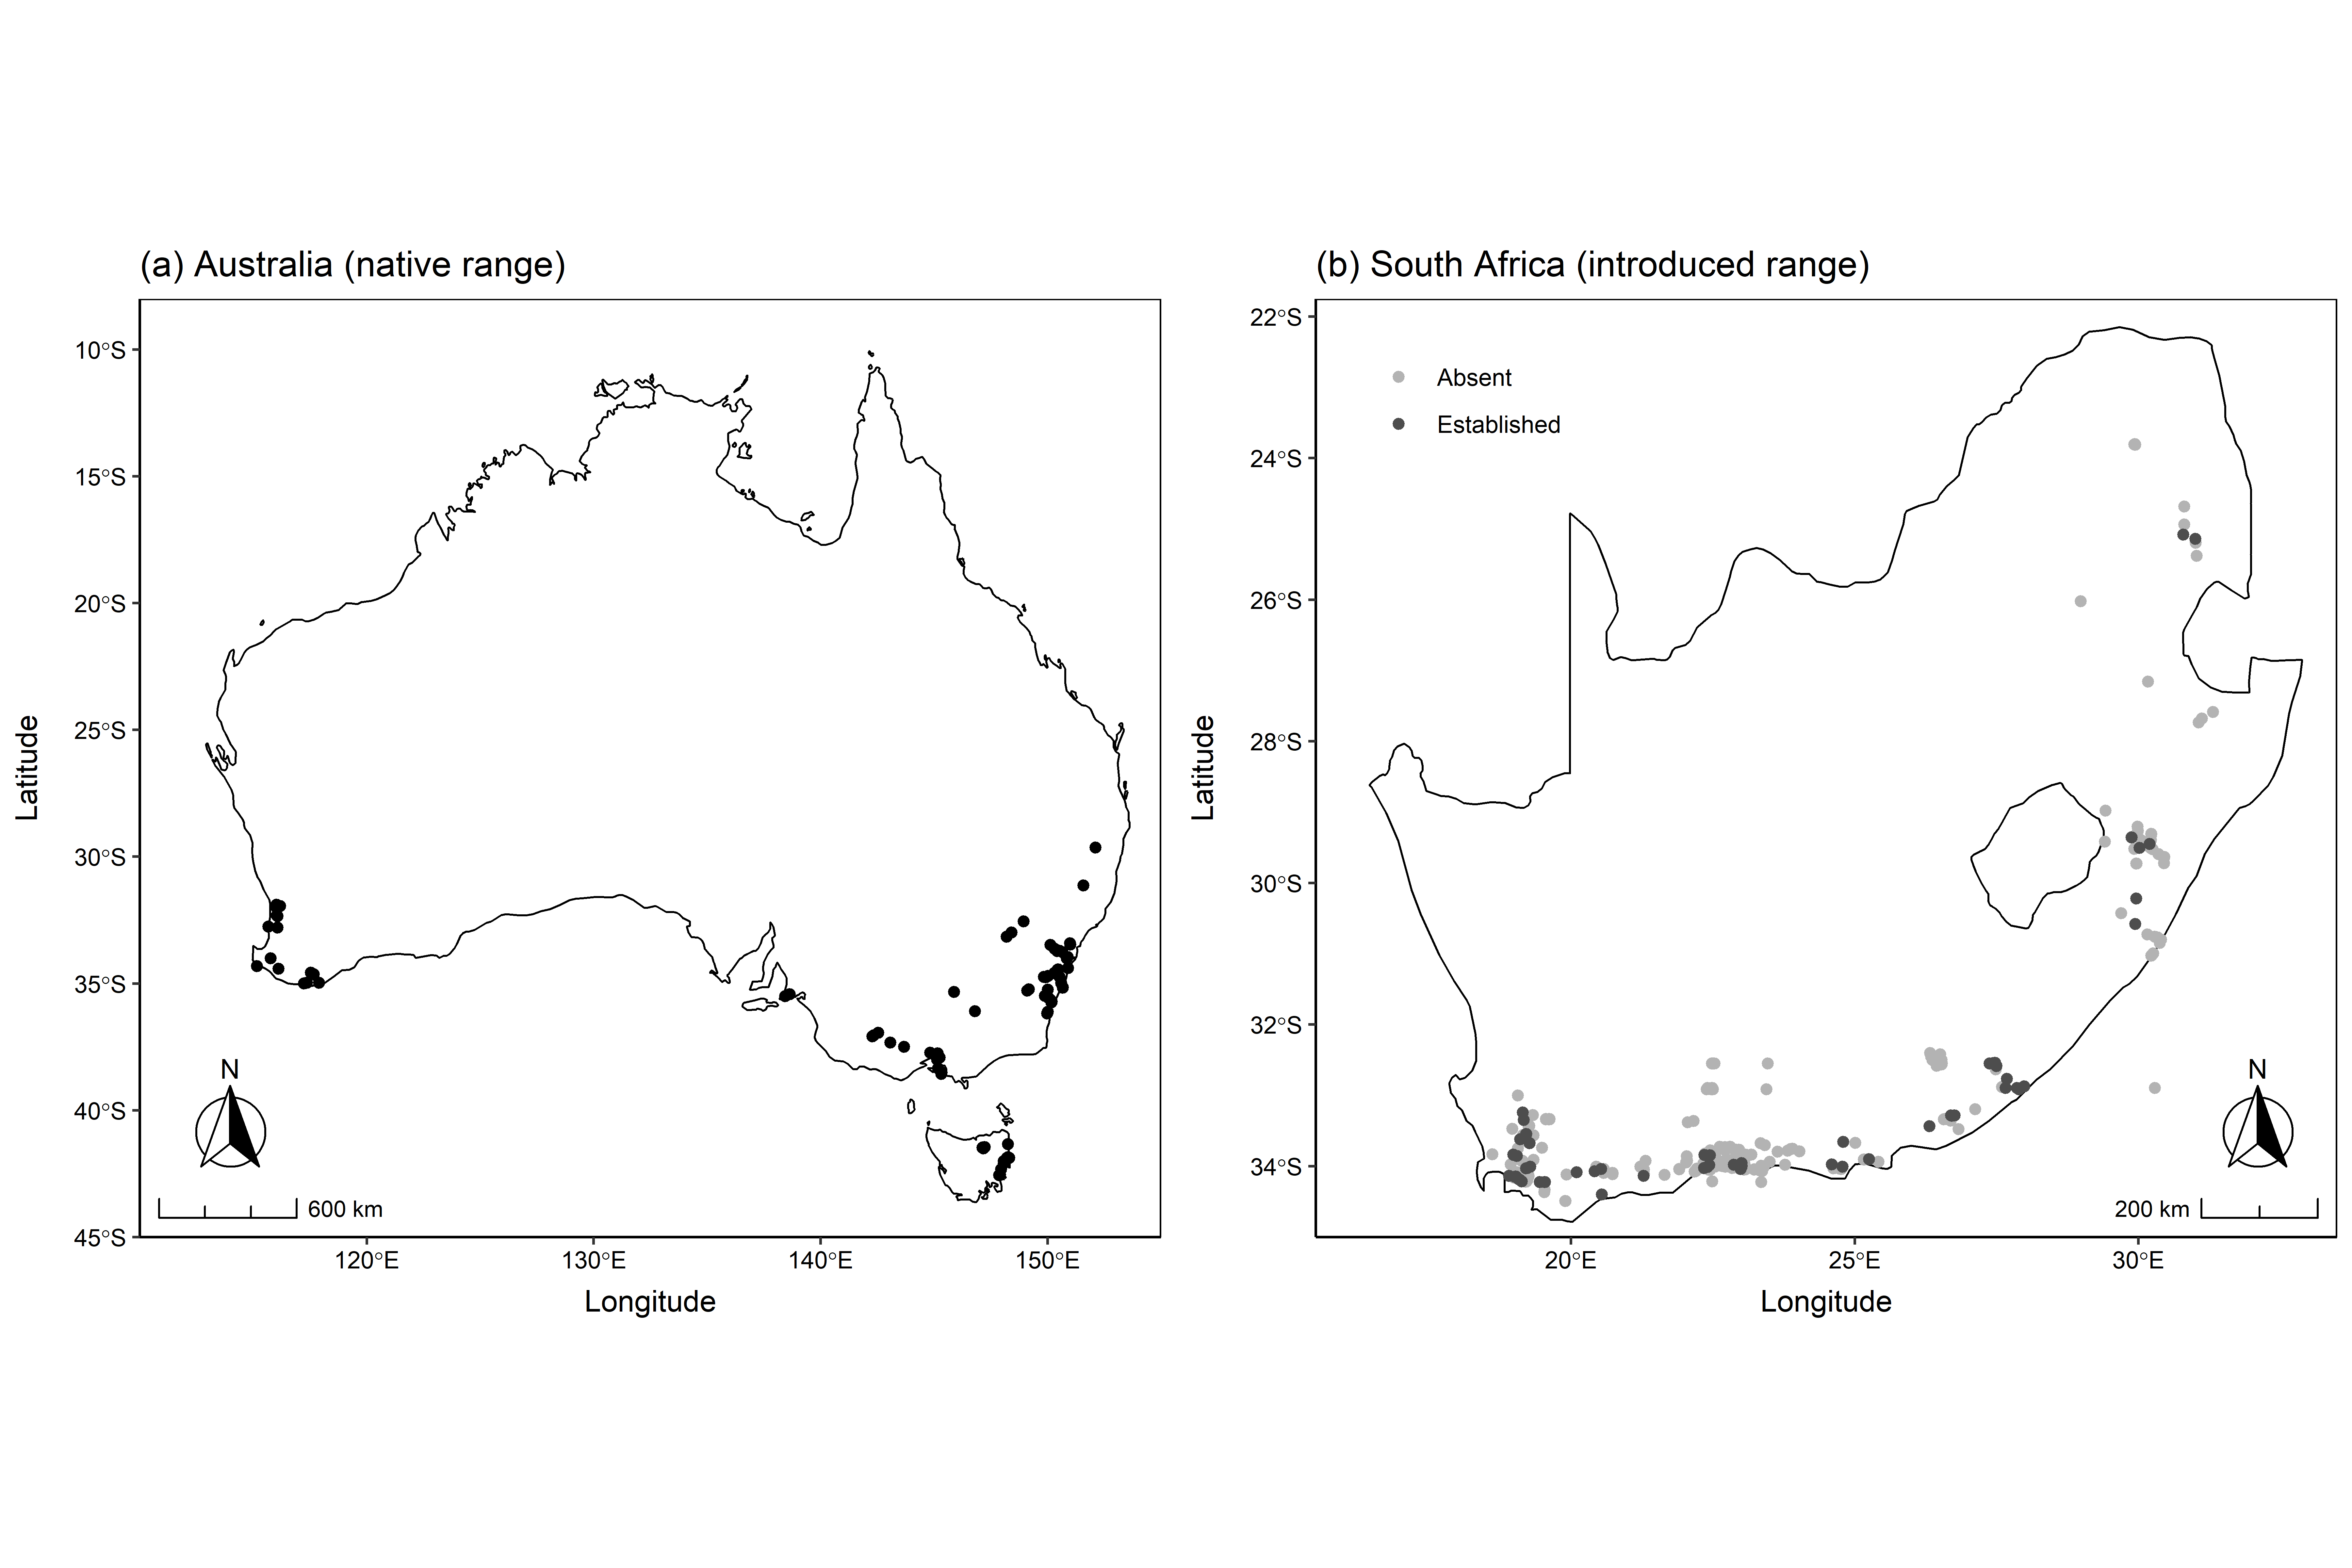
\includegraphics{C:/Users/s1900332/OneDrive - Rhodes University/Manuscripts/MS-Dasinuera-MaxEnt-Transfer/./ms_body/ms_figs/fig_1_distributions.png}

\newpage

\hypertarget{figure-2}{%
\subsection{\texorpdfstring{\emph{Figure 2}}{Figure 2}}\label{figure-2}}

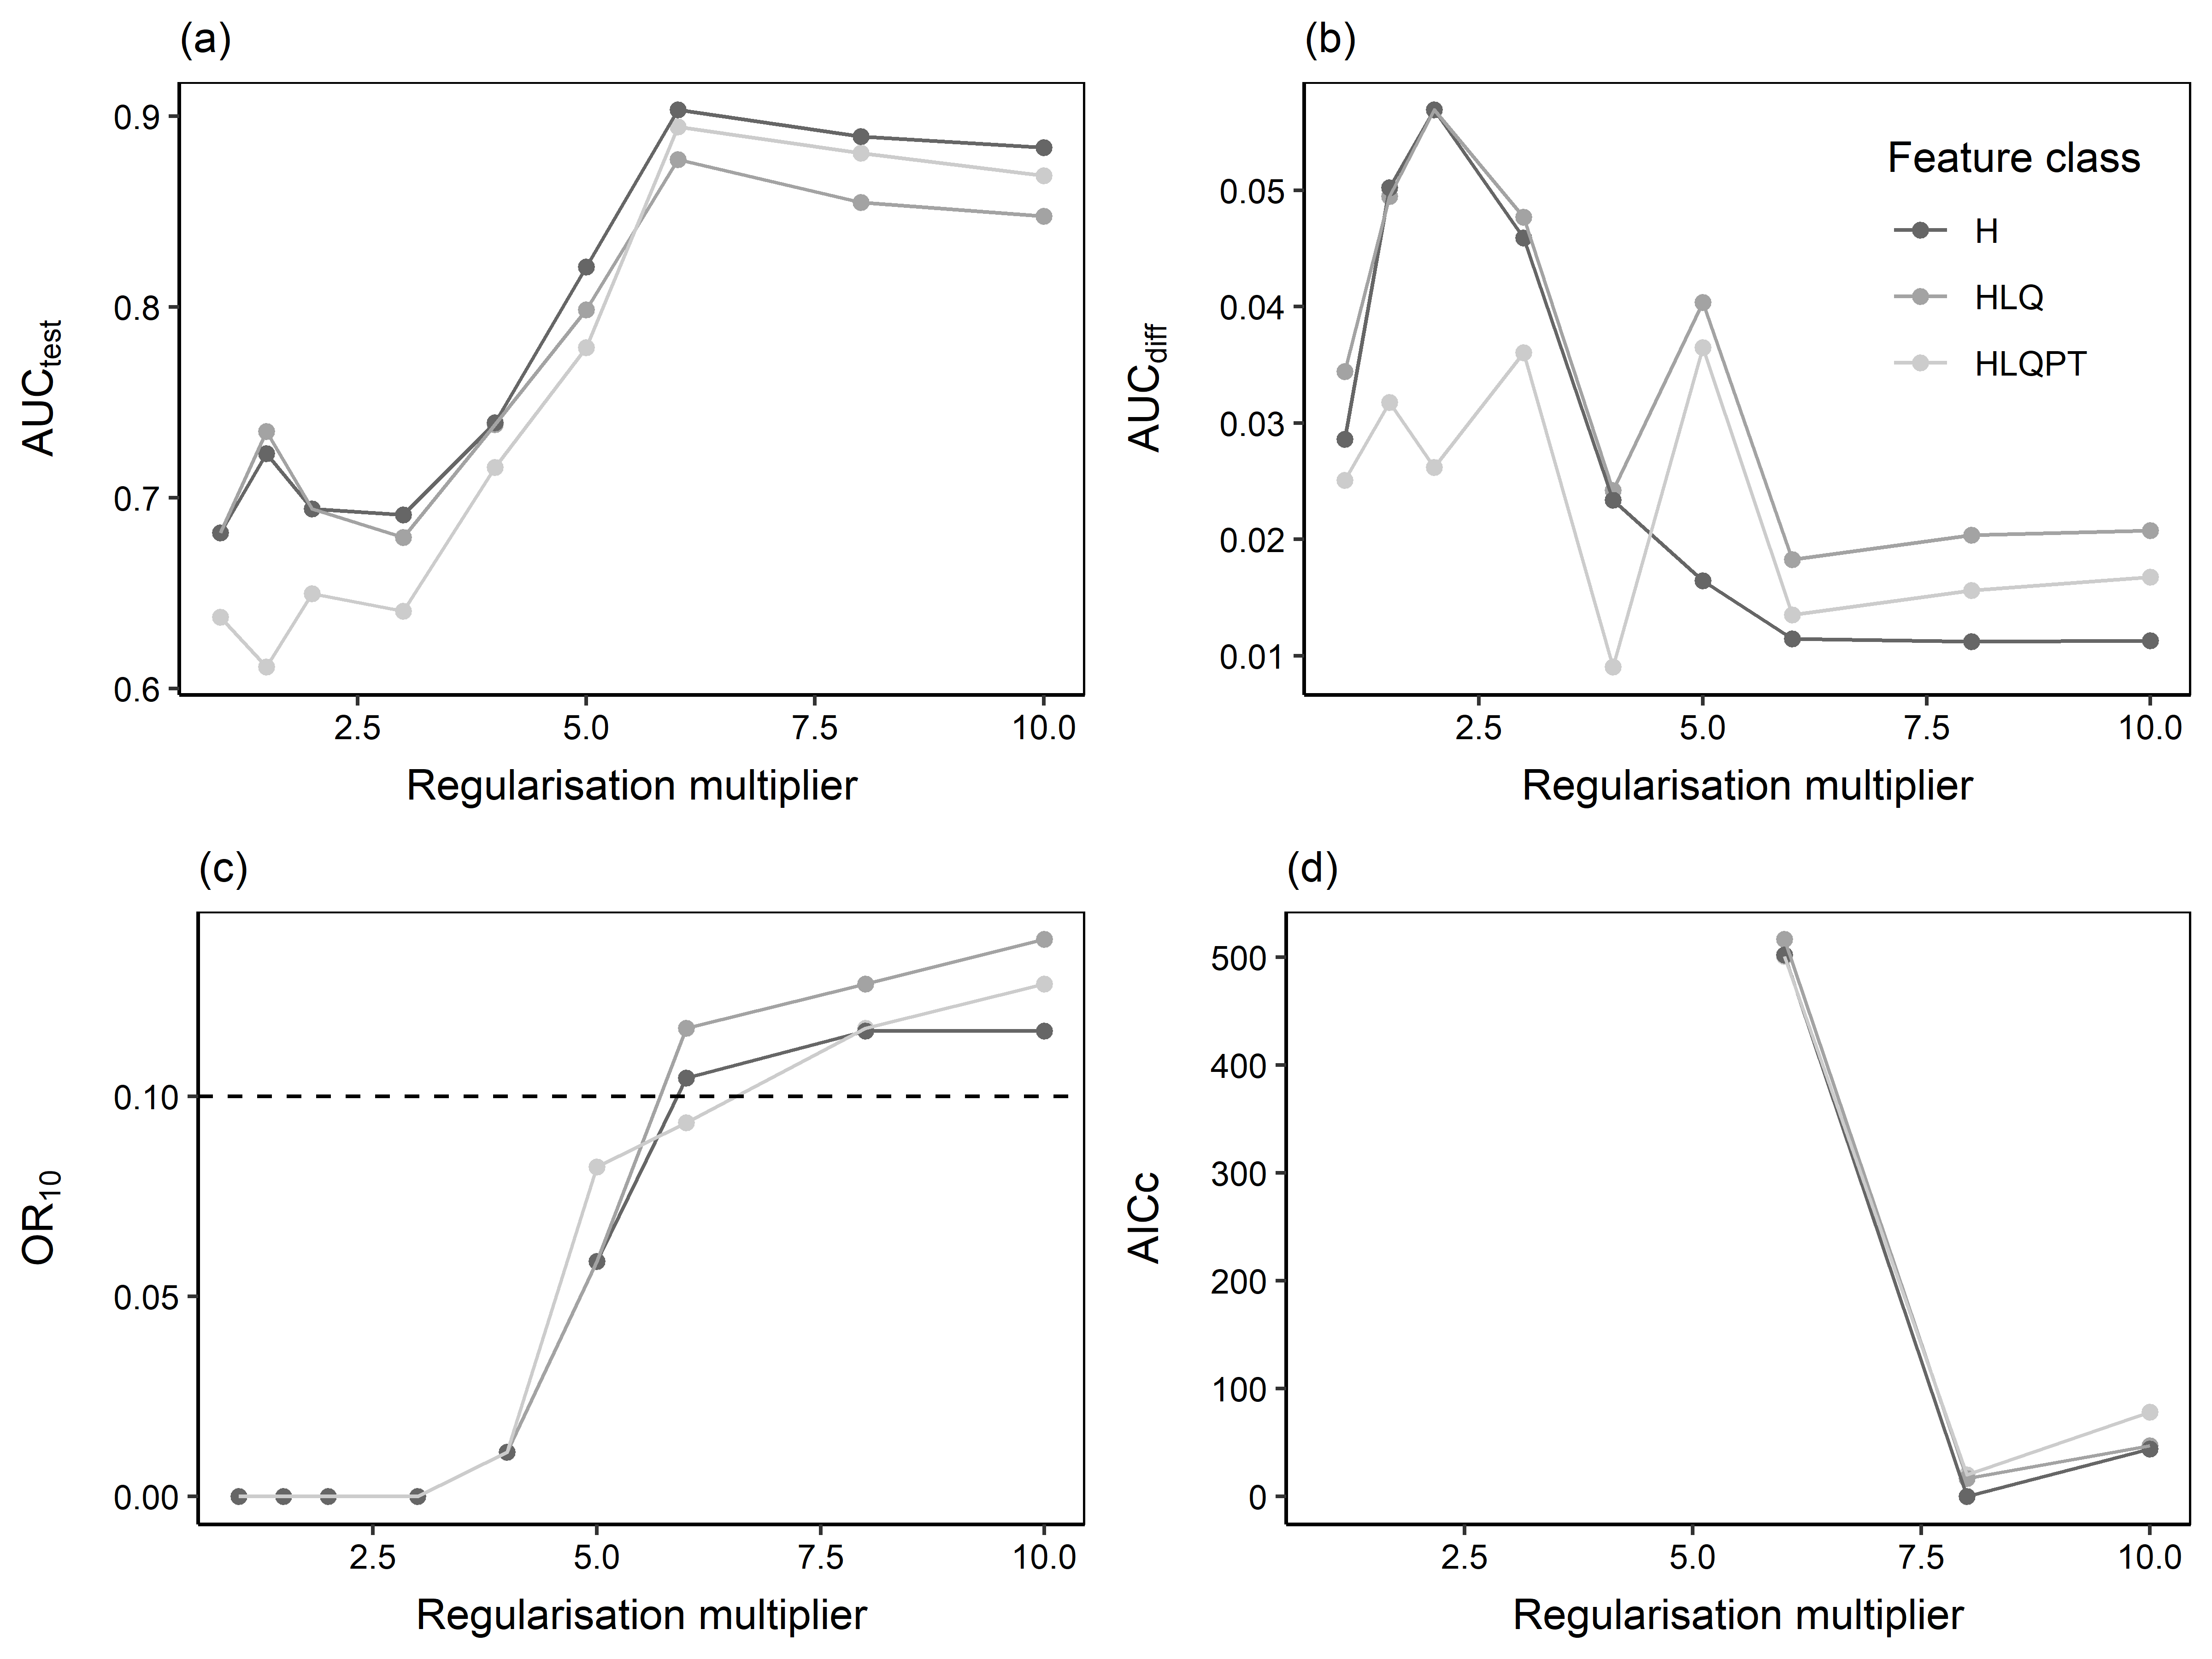
\includegraphics{C:/Users/s1900332/OneDrive - Rhodes University/Manuscripts/MS-Dasinuera-MaxEnt-Transfer/./ms_body/ms_figs/fig_2_model_tuning.png}

\newpage

\hypertarget{figure-3}{%
\subsection{\texorpdfstring{\emph{Figure 3}}{Figure 3}}\label{figure-3}}

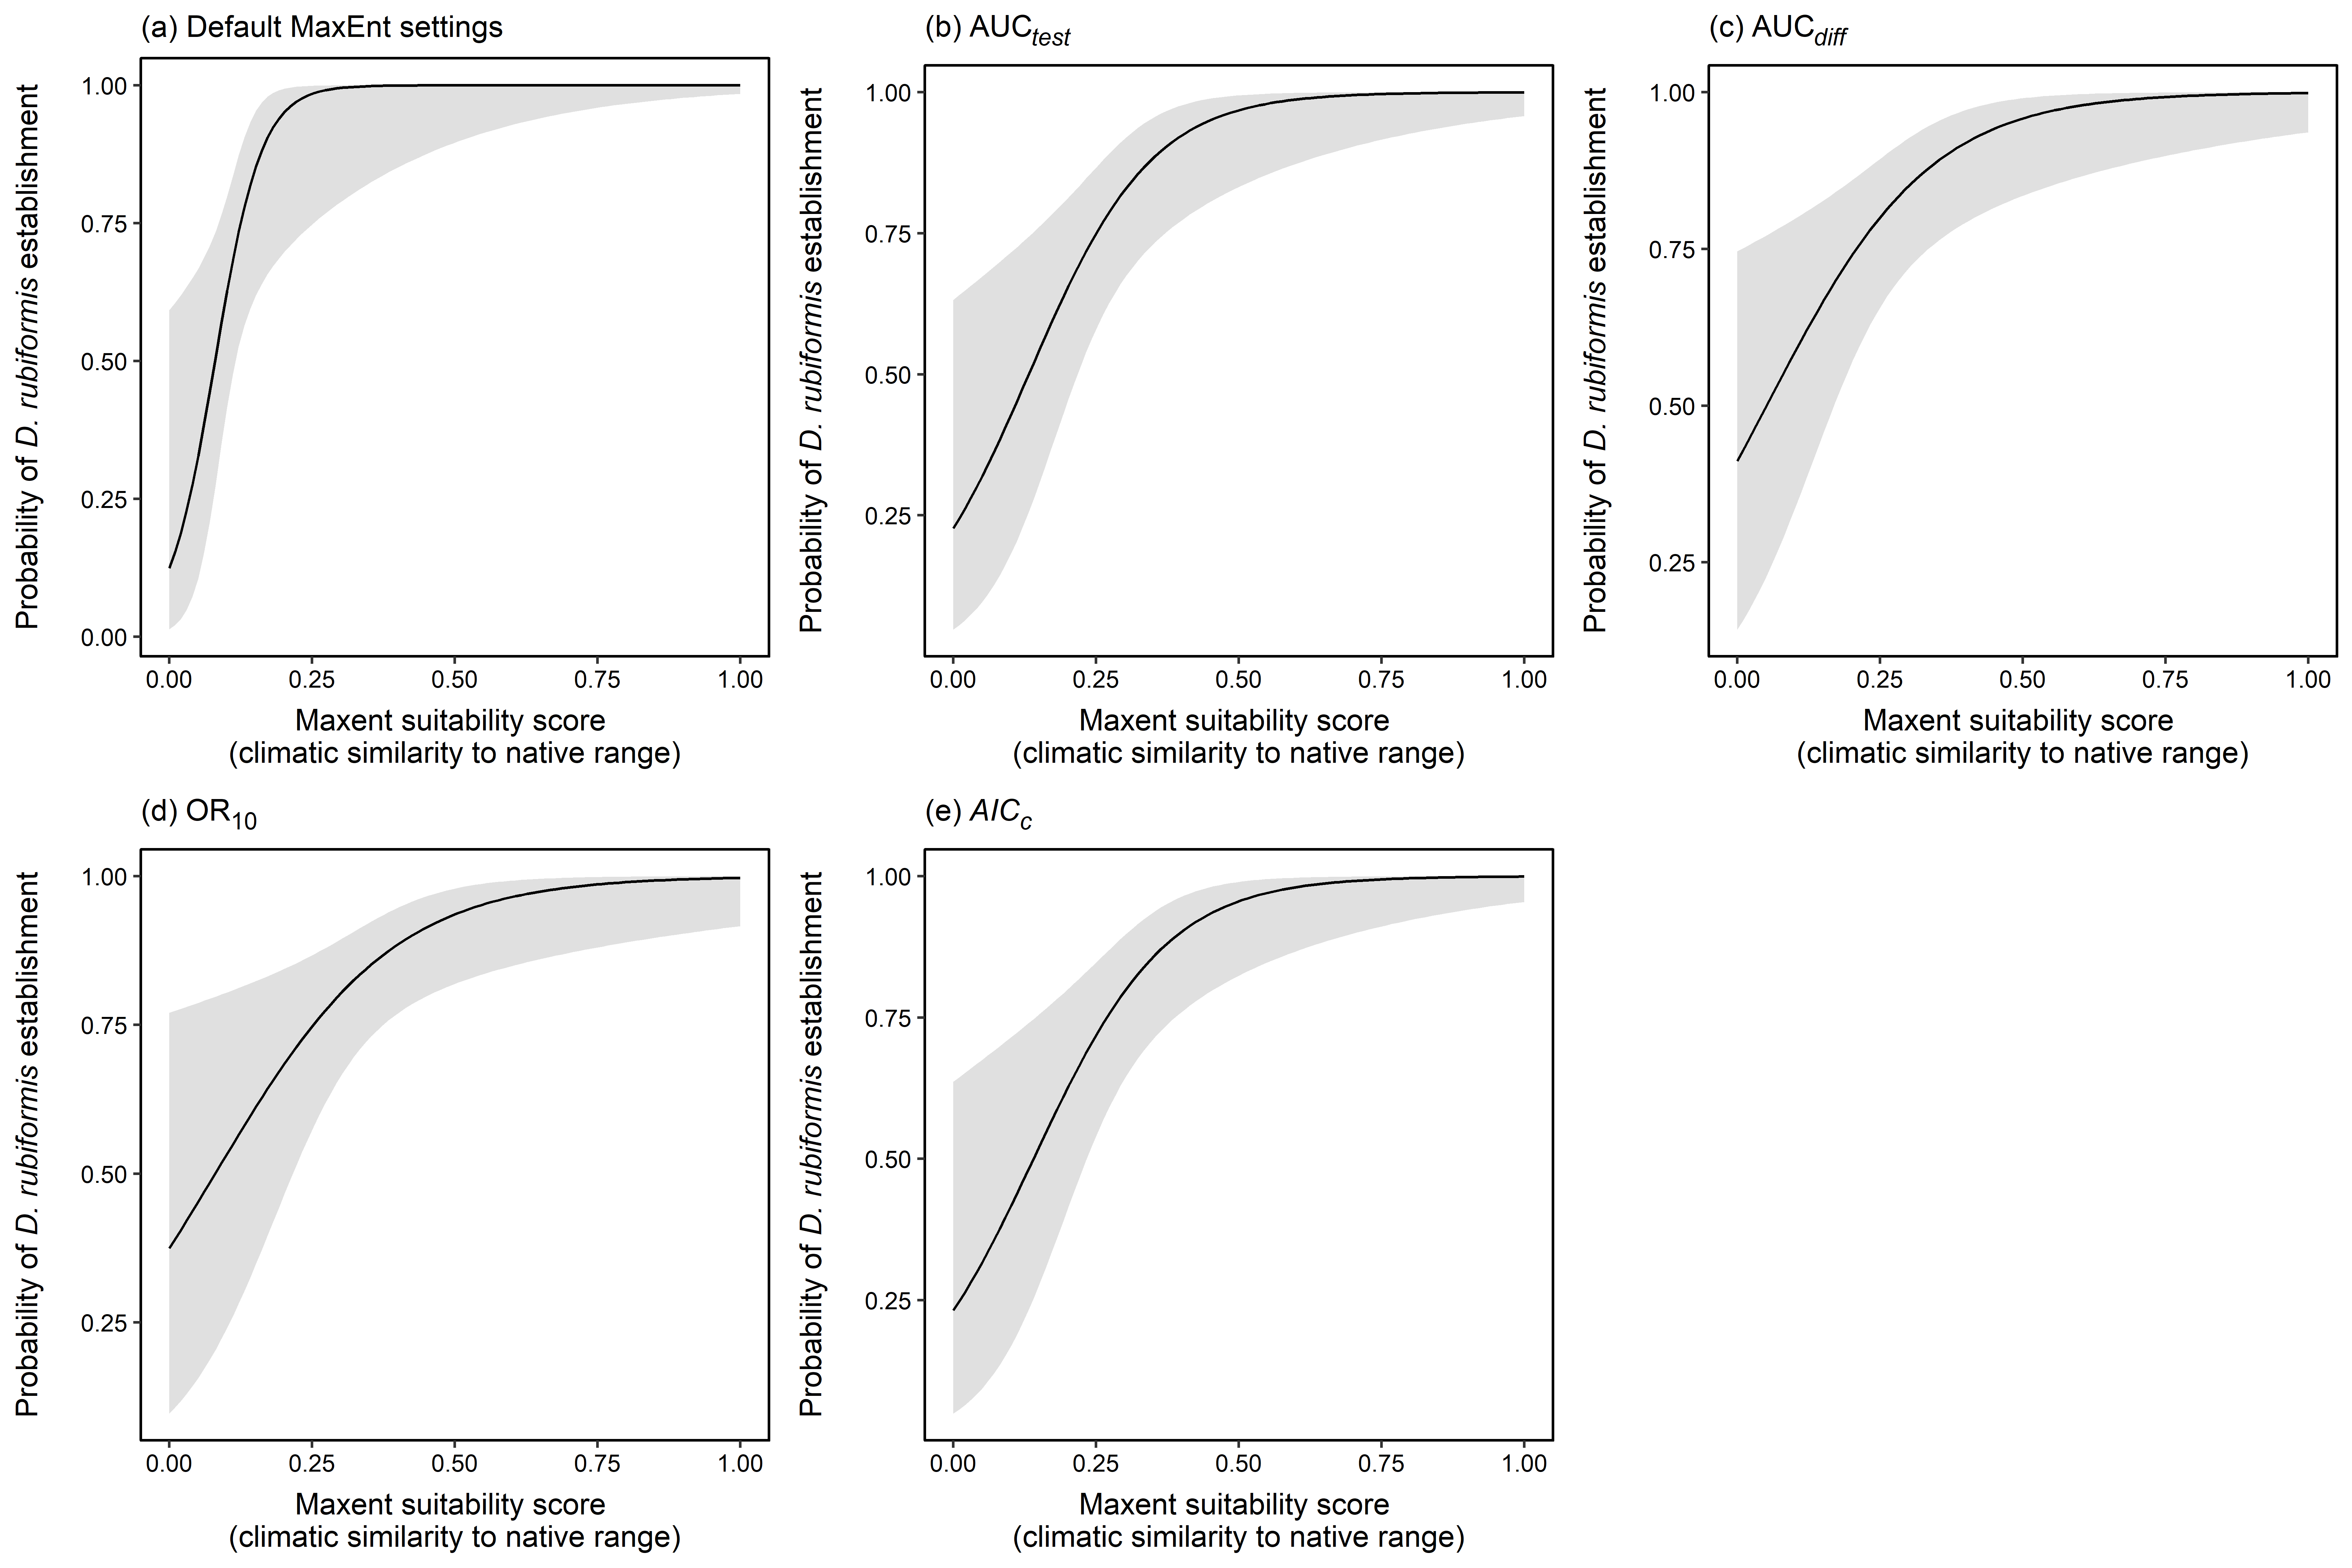
\includegraphics{C:/Users/s1900332/OneDrive - Rhodes University/Manuscripts/MS-Dasinuera-MaxEnt-Transfer/./ms_body/ms_figs/fig_3_logits.png}

\newpage

\hypertarget{figure-4}{%
\subsection{\texorpdfstring{\emph{Figure 4}}{Figure 4}}\label{figure-4}}

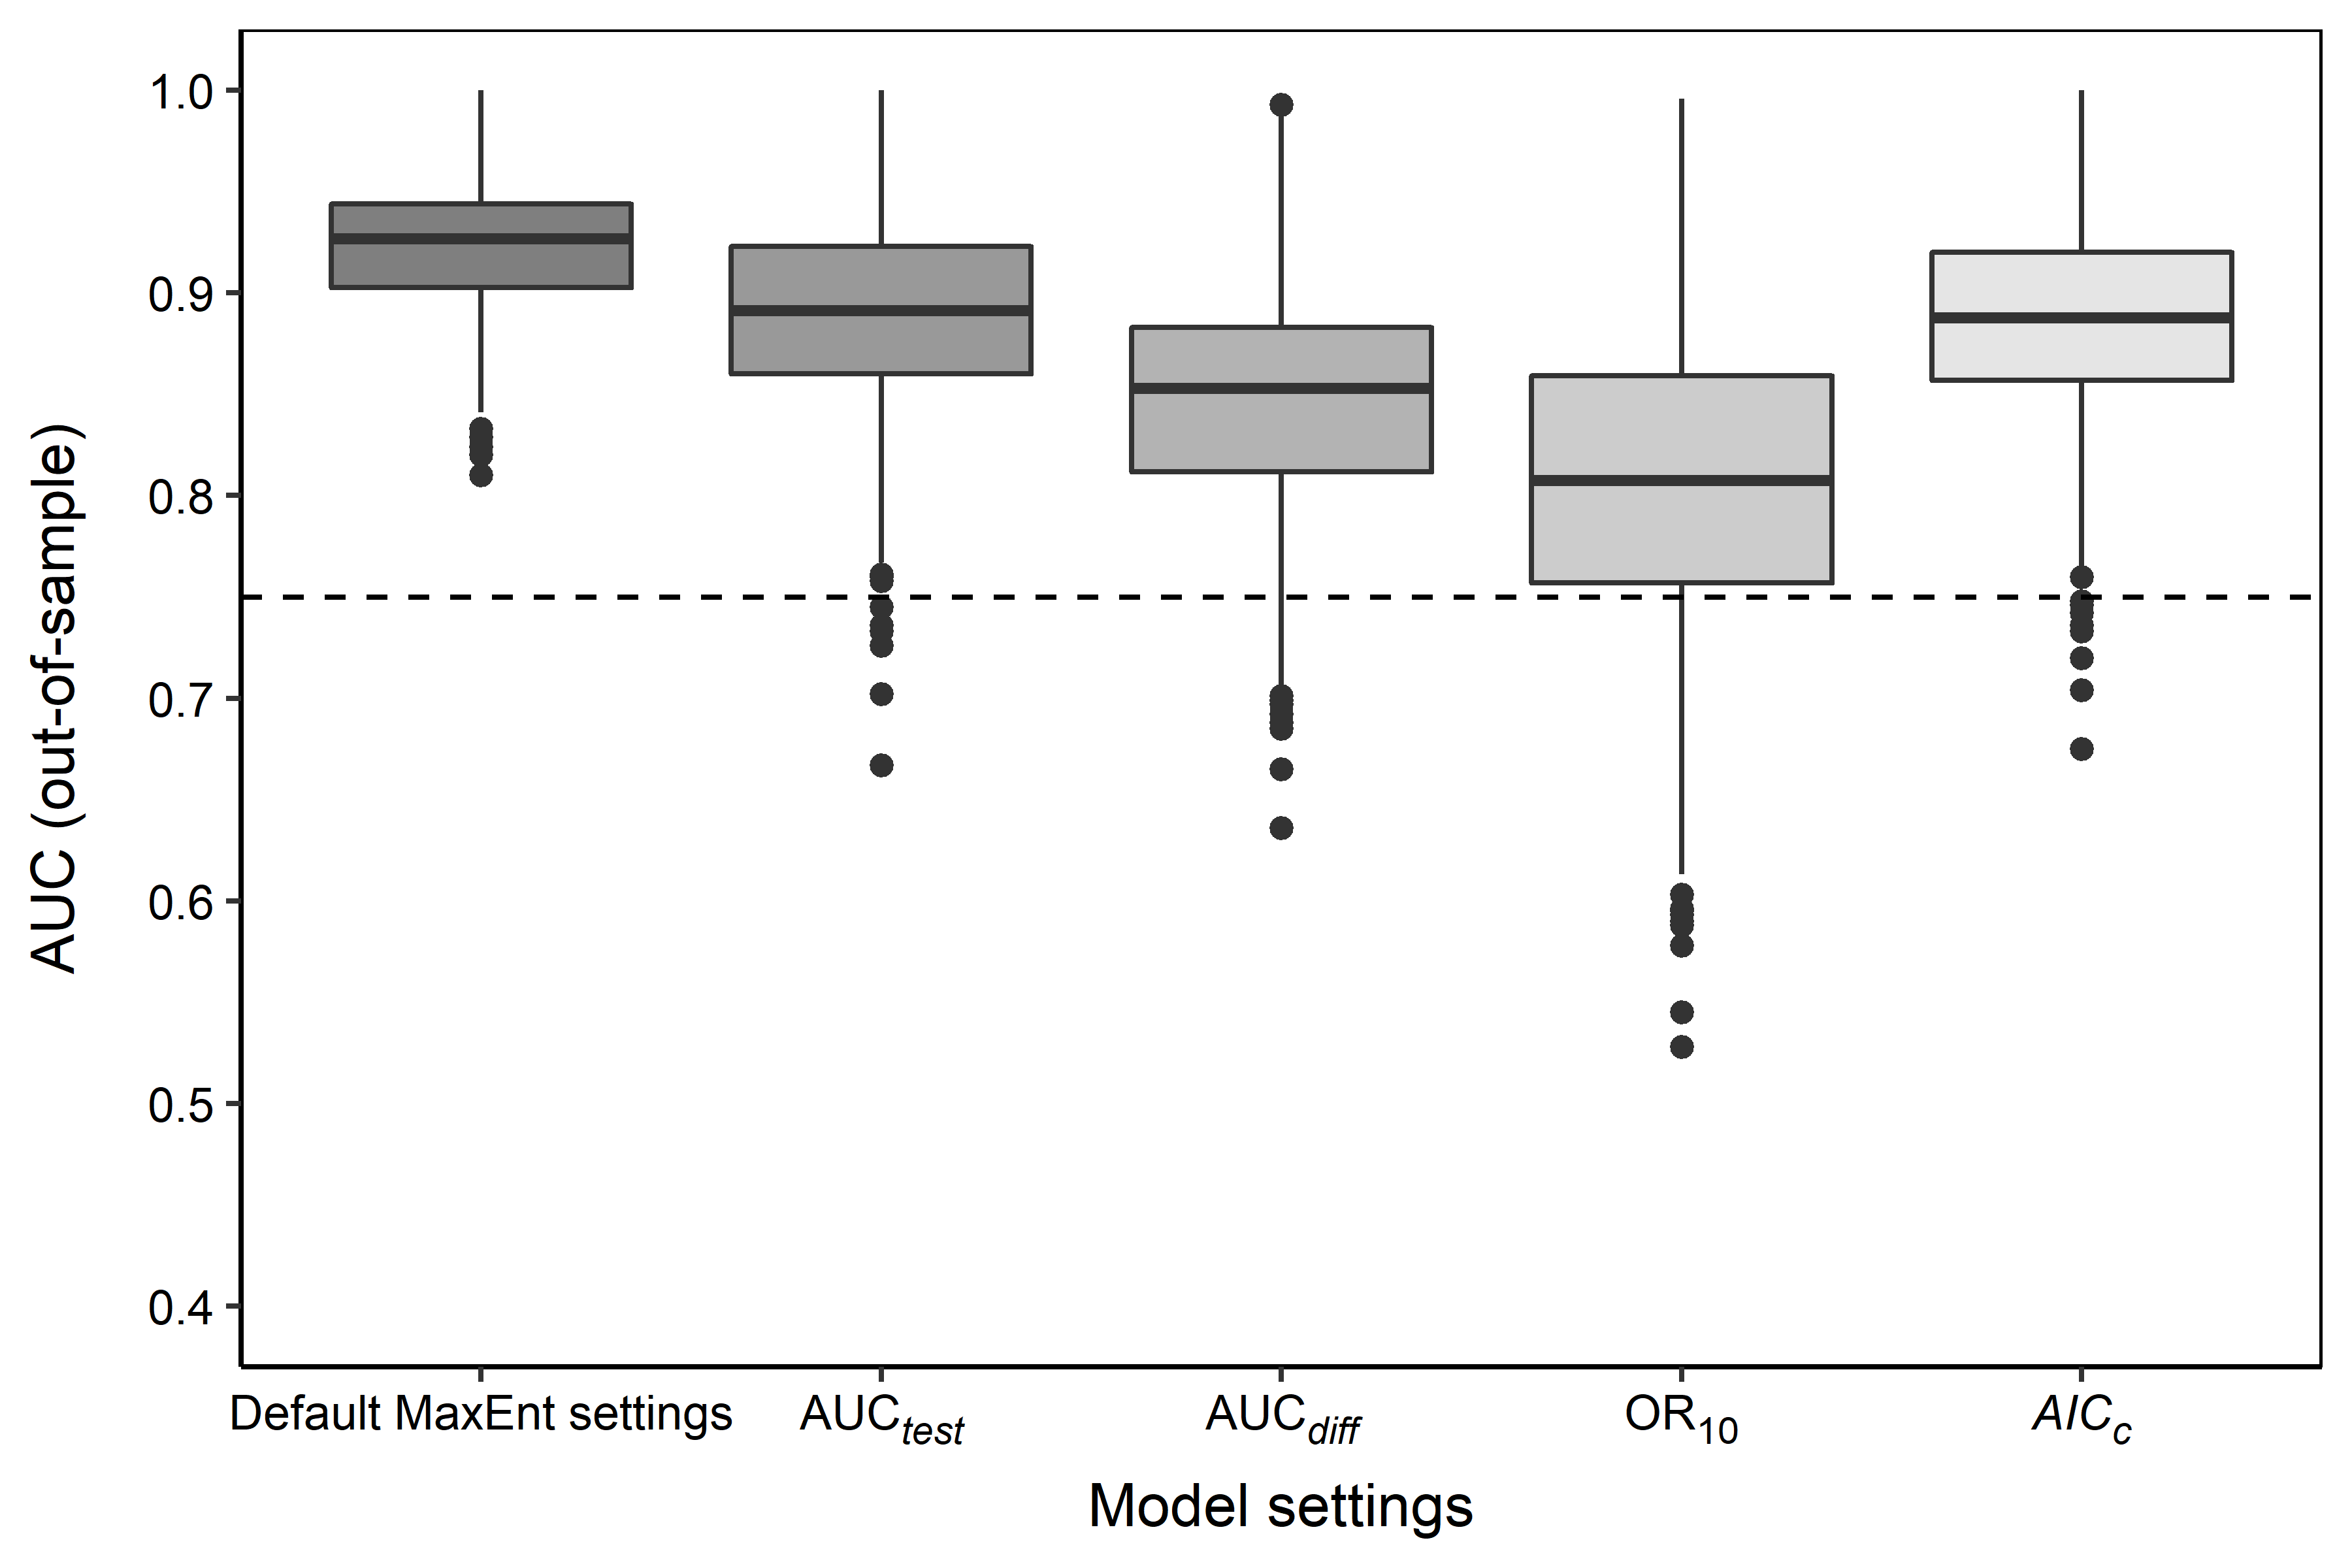
\includegraphics[width=0.8\linewidth,height=0.8\textheight]{C:/Users/s1900332/OneDrive - Rhodes University/Manuscripts/MS-Dasinuera-MaxEnt-Transfer/./ms_body/ms_figs/fig_4_auc}

\newpage

\hypertarget{figure-5}{%
\subsection{\texorpdfstring{\emph{Figure 5}}{Figure 5}}\label{figure-5}}

\includegraphics[width=1\linewidth,height=1\textheight]{C:/Users/s1900332/OneDrive - Rhodes University/Manuscripts/MS-Dasinuera-MaxEnt-Transfer/./ms_body/ms_figs/fig_5_maxent_maps}

\newpage

\hypertarget{figure-6}{%
\subsection{\texorpdfstring{\emph{Figure 6}}{Figure 6}}\label{figure-6}}

\includegraphics{C:/Users/s1900332/OneDrive - Rhodes University/Manuscripts/MS-Dasinuera-MaxEnt-Transfer/./ms_body/ms_figs/fig_6_mess.png}

\newpage

\hypertarget{figure-7}{%
\subsection{\texorpdfstring{\emph{Figure 7}}{Figure 7}}\label{figure-7}}

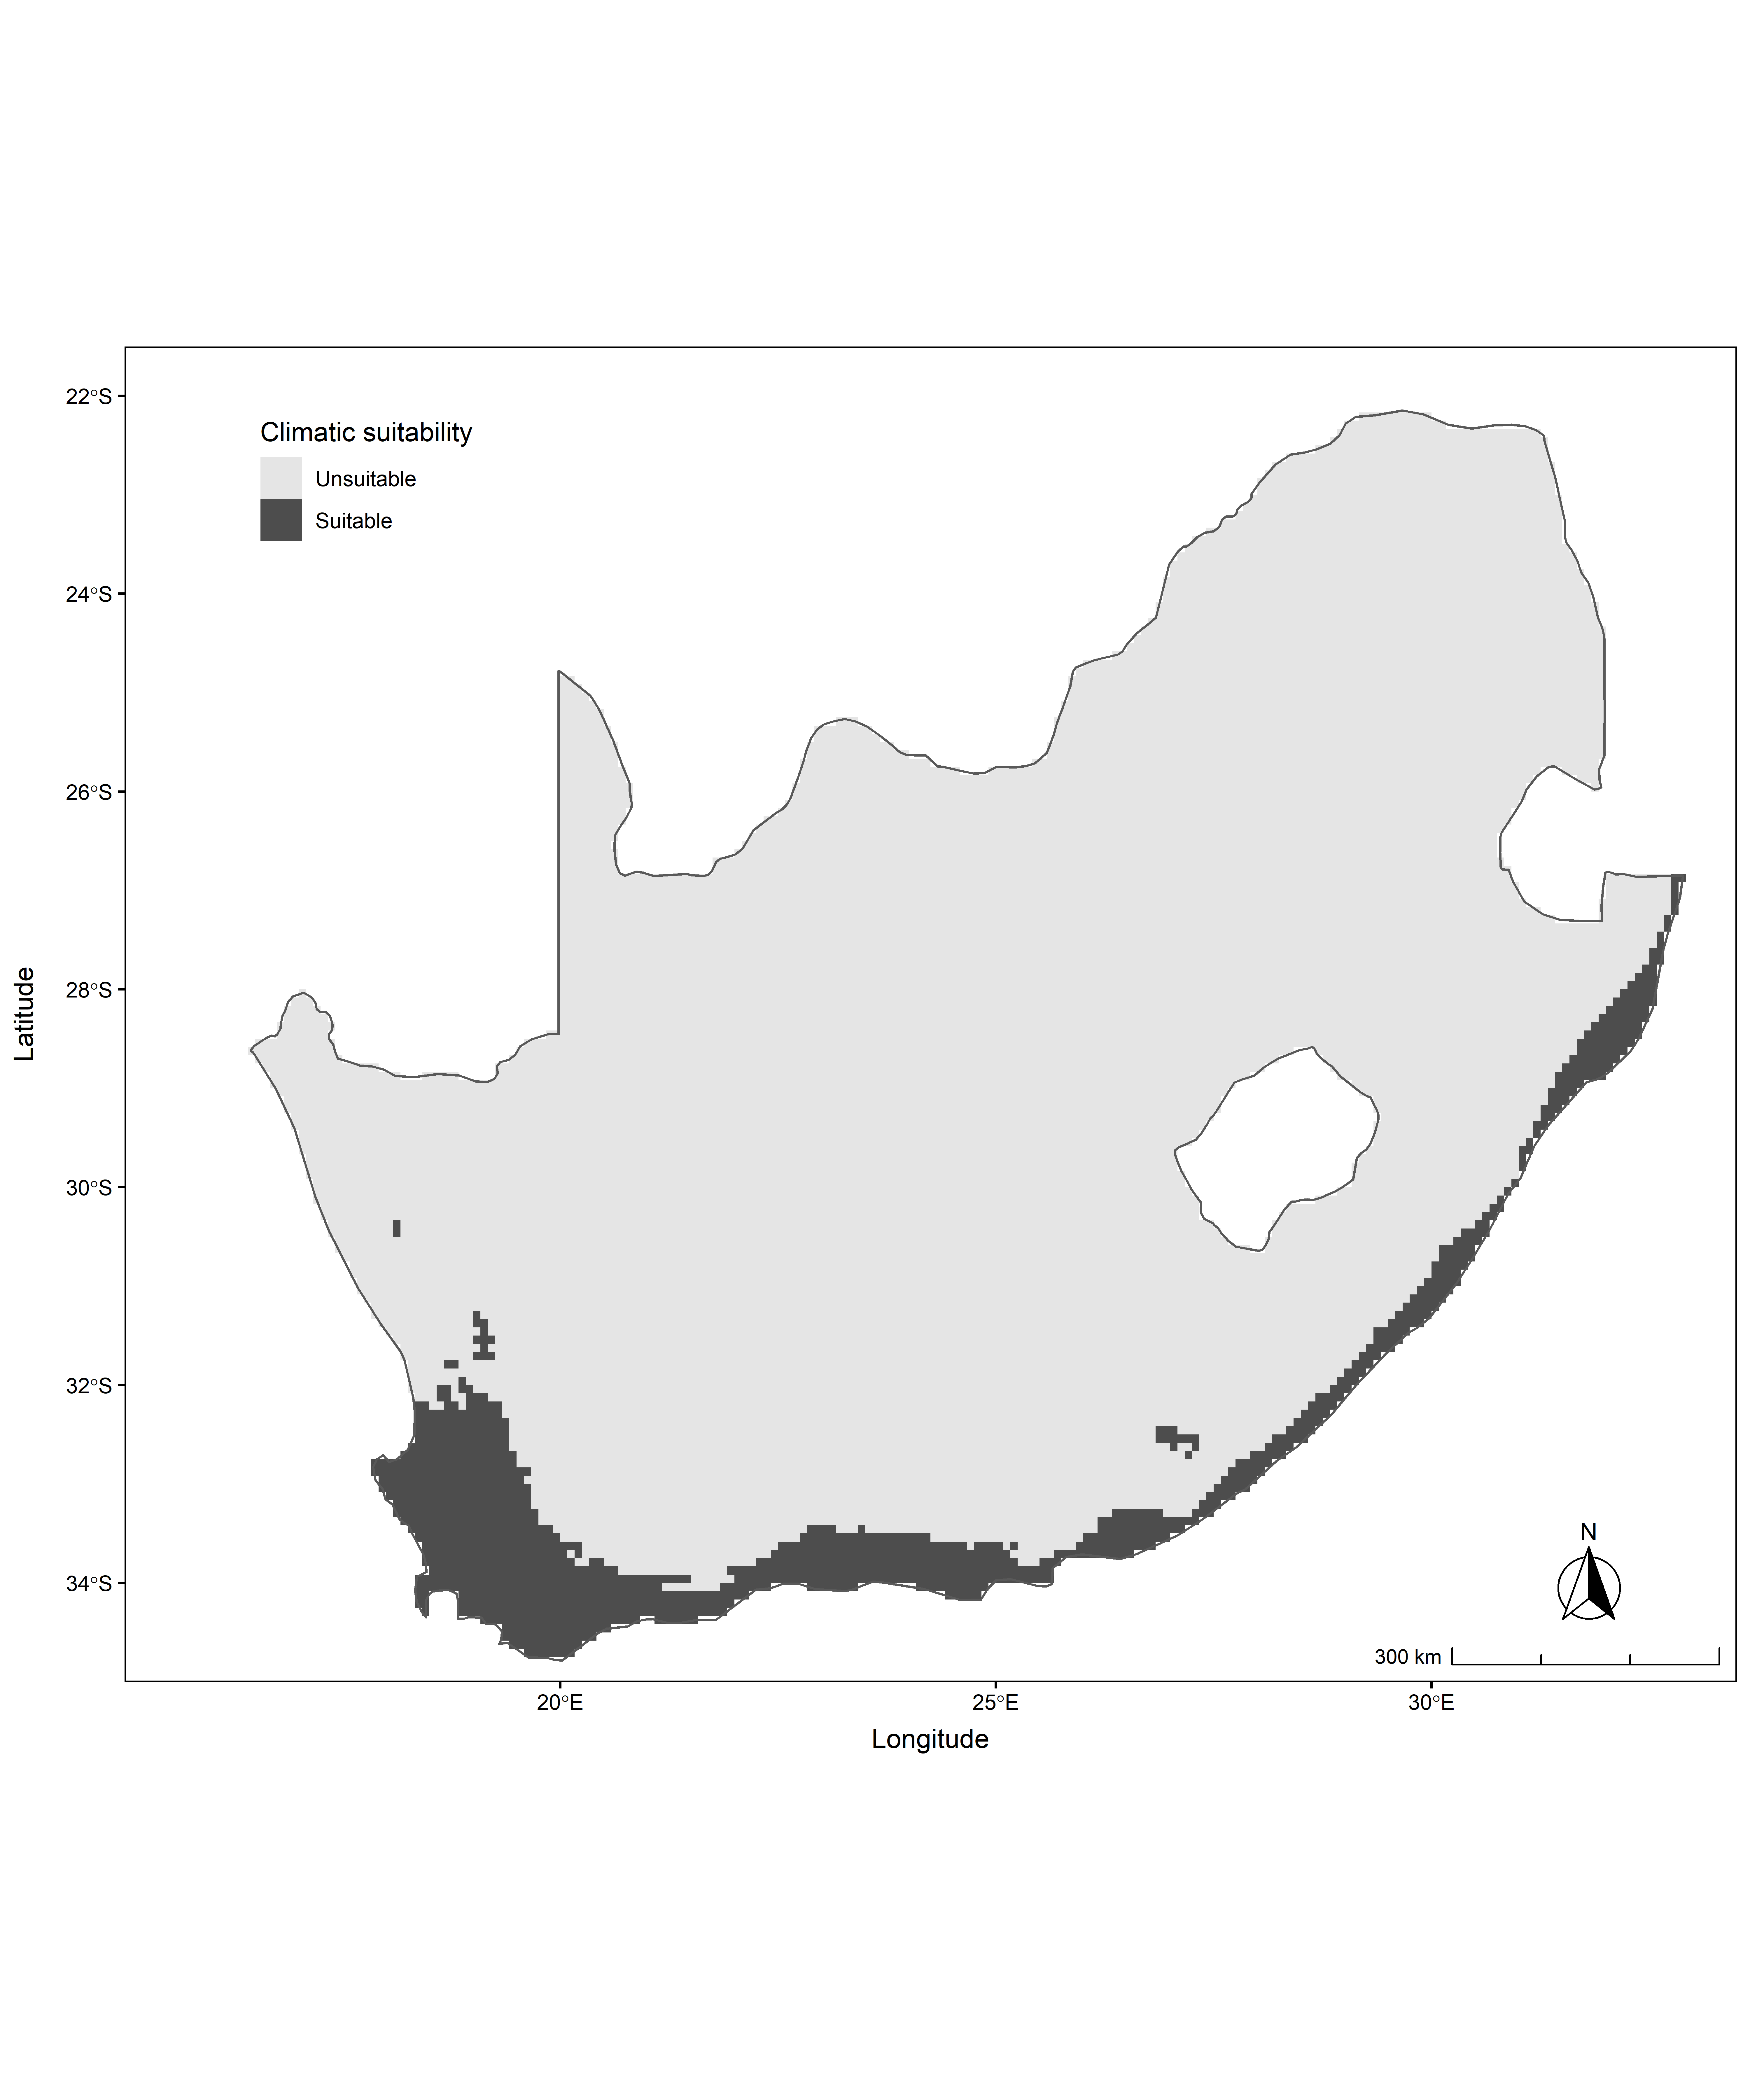
\includegraphics{C:/Users/s1900332/OneDrive - Rhodes University/Manuscripts/MS-Dasinuera-MaxEnt-Transfer/./ms_body/ms_figs/fig_7_biocontrol.png}

\newpage

\textbf{Table 1}

~

\begin{ThreePartTable}
\begin{TableNotes}
\item[a] Adjusted to indicate change in Y for each 1\% unit increase in climatic similarity
\end{TableNotes}
\begin{longtable}[l]{lllll}
\toprule
Model & $\beta$\textsuperscript{a} & $\chi$\textsubscript{2} & d.f. & \textit{P}\\
\midrule
\endfirsthead
\multicolumn{5}{@{}l}{\textit{(continued)}}\\
\toprule
Model & $\beta$\textsuperscript{a} & $\chi$\textsubscript{2} & d.f. & \textit{P}\\
\midrule
\endhead

\endfoot
\bottomrule
\insertTableNotes
\endlastfoot
\cellcolor{gray!6}{Default settings} & \cellcolor{gray!6}{1.11} & \cellcolor{gray!6}{26.21} & \cellcolor{gray!6}{1} & \cellcolor{gray!6}{< 0.001}\\
AUCtest & 1.04 & 17.50 & 1 & < 0.001\\
\cellcolor{gray!6}{AUCdiff} & \cellcolor{gray!6}{1.03} & \cellcolor{gray!6}{12.29} & \cellcolor{gray!6}{1} & \cellcolor{gray!6}{< 0.001}\\
OR10 & 1.02 & 9.01 & 1 & 0.003\\
\cellcolor{gray!6}{AICc} & \cellcolor{gray!6}{1.04} & \cellcolor{gray!6}{16.21} & \cellcolor{gray!6}{1} & \cellcolor{gray!6}{< 0.001}\\*
\end{longtable}
\end{ThreePartTable}





\newpage
\singlespacing 
\end{document}
